\documentclass[11pt,a4paper]{article}
\PassOptionsToPackage{obeyspaces,spaces}{url}

\usepackage[T1]{fontenc}
\usepackage[utf8]{inputenc}
\usepackage{lmodern}
\usepackage[french]{babel}
\usepackage[a4paper,margin=2.5cm]{geometry}
\usepackage{amsmath,amssymb}
\usepackage{graphicx}
\usepackage{booktabs}
\usepackage{tabularx}
\usepackage{longtable}
\usepackage{array}
\usepackage{xcolor}
\usepackage{microtype}
\usepackage{csquotes}
\usepackage[backend=biber,style=numeric-comp,sorting=nyt,maxbibnames=4,giveninits=true]{biblatex}
\usepackage[hidelinks]{hyperref}
\usepackage{cleveref}

\addbibresource{rockim.bib}
% Le champ note de rockim.bib porte la provenance interne de chaque entree :
% utile au depot, pas au lecteur de la bibliographie.
\DeclareSourcemap{\maps[datatype=bibtex]{\map{\step[fieldset=note,null]}}}

\graphicspath{{figures/}}

% Cle de configuration ou chemin du depot, en machine a ecrire.
\urlstyle{tt}
\def\UrlBreaks{\do\/\do\_\do\-\do\.}
\DeclareRobustCommand{\cle}[1]{\path{#1}}
% Figure a produire (encadre rouge) : hauteur, contenu attendu, calcul necessaire.
\newcommand{\figaproduire}[3]{%
  \begin{center}\fcolorbox{red}{white}{\begin{minipage}[c][#1][c]{0.9\linewidth}
  \centering\small Figure à produire.\\[0.5ex] Contenu attendu : #2\\[0.5ex]
  Calcul ou essai nécessaire : #3\end{minipage}}\end{center}}

\crefname{section}{section}{sections}
\crefname{figure}{figure}{figures}
\crefname{table}{tableau}{tableaux}
\crefname{appendix}{annexe}{annexes}

\setlength{\parskip}{0.4ex}
\setlength{\emergencystretch}{2em}
\renewcommand{\arraystretch}{1.15}

\title{rockim : ce que fait le code, comment il a été vérifié et ce qu'il reste à valider\\[1ex]
\large Rapport-guide à l'intention des encadrants}
\author{Thèse forage percussif, granite de Red Bohus}
\date{6 octobre 2026\\[0.5ex]\small État du dépôt \cle{Fuzquial/rockim}, commit \cle{f0209ef} du 4 octobre 2026}

\begin{document}
\maketitle

\section*{Synthèse}
\addcontentsline{toc}{section}{Synthèse}

rockim est un code de calcul écrit pendant la thèse, en C++ avec la seule bibliothèque Eigen, pour simuler l'impact d'un insert en carbure sur une roche. Il implémente la méthode combinée éléments finis et éléments discrets (FDEM) de la lignée de Munjiza~\cite{munjiza2004fdem} : la roche est découpée en tétraèdres élastiques reliés par des joints cohésifs qui s'endommagent puis rompent, et les fragments libérés interagissent par contact frottant. Depuis la décision du 14 août 2026, le développement porte sur les modes FDEM 2D et 3D ; les modes éléments finis continus et éléments discrets sont gelés, et la production 3D calibrée de la thèse reste confiée à Abaqus avec les VUMAT de la thèse.

Le code résout correctement plusieurs de ses briques, et ces vérifications se rejouent en une commande. Le contact par potentiel conserve l'énergie d'une collision élastique à $2\times10^{-8}$ près en 3D ; l'algèbre du contact d'outil en vitesse est juste à $2{,}2\times10^{-16}$ ; une barre en traction donne l'allongement $\sigma L/E$ à $0{,}03~\%$ ; les 26 contrôles à charge nulle ne rompent aucun joint ; le bilan d'énergie à sept postes ferme à l'arrondi en élastique. Une onde de compression dans une barre est reproduite par le solveur éléments finis 3D avec une célérité juste à $0{,}05~\%$ et un ordre de convergence observé de $1{,}58$. Un bloc qui glisse jusqu'à l'arrêt s'arrête à $1{,}74~\%$ de la distance exacte avec le contact par potentiel.

Ces mêmes bancs ont révélé deux biais qui touchent directement l'impact. Avec des joints présents dès l'origine et une pénalité de 20 fois $E/h$, l'onde est ralentie de $2{,}9$ à $3{,}2~\%$ quel que soit le maillage ; la loi de correction mesurée fixe la pénalité à au moins $0{,}62/\varepsilon$ pour un biais $\varepsilon$. Le contact par pénalité nœud-face, réglage par défaut, fait basculer le bloc glissant au lieu de le laisser glisser ; le contact par potentiel est donc requis dès que deux corps glissent l'un sur l'autre.

La reproduction d'articles est partielle. Sur l'impact d'un insert sur le calcaire de St Anne (Yang et al. 2025~\cite{yang2025validation}), un calcul complet de $300~\mu$s place la contrainte au taillant, la vitesse d'indentation, le rayon du cratère et la fin de la phase de charge à 6 à $12~\%$ des valeurs publiées, avec un bilan d'énergie fermé à $1{,}5\times10^{-7}~\%$. L'enfoncement est trop grand de $17~\%$, la masse de fragments de $87~\%$, et le rebond n'est pas mesuré. Cette comparaison n'est pas indépendante du calage : la loi de joint et la pénalité ont été choisies pendant la même campagne. L'impact sur le granite de Kuru (Yang et al. 2026~\cite{yang2026pulverisation}) n'est pas reproduit : la pulvérisation reste quasi inactive et la loi de joint du code de référence, transcrite telle quelle, crée de l'énergie.

Rien n'est validé au sens strict, c'est-à-dire contre un essai qui n'a pas servi au calage. Les parties III et IV de la campagne de vérification et validation sont vides, sept bancs sont préparés avec leurs critères écrits avant calcul mais n'ont tourné qu'en essai de fumée, et la calibration sur le granite de Red Bohus n'est pas conclue. Les résultats dépendent du nombre de fils de calcul, à environ $2~\%$ sur les pics.
\clearpage

\tableofcontents
\clearpage
\section{Objet et périmètre du code}
\label{sec-objet}

\subsection{Le problème physique}

Le forage percussif fragmente la roche par une succession de chocs : un piston frappe un taillant (le bit), l'onde de compression traverse le bit et les inserts en carbure de tungstène la transmettent à la roche, qui se fissure, se broie et éjecte des fragments sous chaque insert. rockim simule ce problème à l'échelle d'un insert : l'élasticité du volume, la fissuration par des joints cohésifs, le contact frottant entre fragments, l'effet de la vitesse de déformation sur la résistance, la pulvérisation du volume et le bilan d'énergie de tout le système (\cle{LISEZ_MOI.md}, l.~6-13).

Deux familles de données servent de cibles, et elles ne portent pas sur la même roche. Les essais d'impact à insert unique d'Imperial College et de Mines Paris-PSL, publiés par Yang et al.~\cite{yang2025validation,yang2026pulverisation}, portent sur le calcaire de St Anne, le grès de Rhune et le granite de Kuru Grey (\cle{specs/005-impact-insert-yang/spec.md}, l.~9-24). Les essais quasi statiques sur le granite de Red Bohus, matériau de la thèse, fournissent une résistance en compression simple de $126{,}6 \pm 21{,}4$~MPa, une résistance brésilienne de $10{,}27$~MPa, un module de $77{,}7$~GPa et un coefficient de Poisson de $0{,}29$~\cite{dumoulin2024data} (\cle{calibration_redbohus/README.md}, l.~18-25). Aucune donnée d'impact sur le Red Bohus n'alimente aujourd'hui rockim.

\subsection{Raison d'être d'un code maison}

Le dépôt ne contient pas de justification écrite du choix de développer un code plutôt que d'utiliser un code existant. Les documents fixent quatre objectifs au code : une parité structurelle avec le code de l'article de référence (MultiFracS, lignée Munjiza), la reproduction d'un impact validable contre le banc de Mines Paris, la robustesse et la vitesse (\cle{ROADMAP_rockim.md}, l.~3-6). Le guide d'utilisation le présente comme un bac à sable d'exploration, de calibration et de figures, la production 3D calibrée restant confiée à Abaqus et aux VUMAT (\cle{GUIDE_rockim.md}, l.~465-466).

Le code de référence des articles de Yang et al., Solidity (Imperial College, licence LGPL version 3), n'est pas redistribué dans rockim. rockim en transcrit des conventions, ligne à ligne pour certaines, en citant les fichiers sources de Solidity. Le dépôt public de rockim n'a pas de licence alors qu'il contient ces transcriptions : ce point juridique est ouvert (\cle{HANDOFF_2026-10-03.md}, l.~192-193). Une contrainte du doctorant distingue aussi rockim de Solidity : garder l'insertion adaptative des joints (Yan et al. 2023~\cite{yan2023adaptive}), là où Solidity place les joints partout dès l'origine.

\subsection{Les modes de calcul}

Six solveurs partagent une interface commune et se choisissent par la clé \cle{mode} (\cref{tab-modes}). Chaque mode accepte plusieurs scénarios de chargement : \cle{percussion} (impacteur libre), \cle{shear} (coupe par un outil traîné à profondeur imposée, dont un couteau PDC en 2D et en 3D), \cle{tension} (traction, ou compression simple et triaxiale par platines et confinement), \cle{loads} (charges par groupes de nœuds, ajouté le 3 octobre 2026), \cle{brazilian} et \cle{shpb} en FDEM 2D seulement, et \cle{jointbench} (banc d'un joint isolé) en FDEM 3D. Douze sous-commandes \cle{selftest-*} vérifient des briques sans maillage (\cref{sec-verification}).

\begin{table}[htbp]
\centering
\caption{Les six solveurs de rockim et leur statut depuis la décision de périmètre du 14 août 2026.}
\label{tab-modes}
\begin{tabularx}{\linewidth}{@{}l X l l@{}}
\toprule
mode & modèle & rupture & statut \\
\midrule
\cle{fem} & éléments finis 2D, déformation plane, triangles à déformation constante & endommagement et érosion & gelé \\
\cle{fem3d} & tétraèdres co-rotationnels, lois de volume au choix & endommagement et érosion & gelé, enrichi \\
\cle{dem}, \cle{dem3d} & particules liées (modèle à liaisons parallèles) & rupture des liaisons & gelé \\
\cle{fdem} & FDEM 2D, grains de Voronoï possibles & joints cohésifs explicites & actif \\
\cle{fdem3d} & FDEM 3D, tétraèdres, grains de Voronoï possibles & joints cohésifs triangulaires & actif \\
\bottomrule
\end{tabularx}
\end{table}

La décision du 14 août 2026 concentre le développement sur \cle{fdem} et \cle{fdem3d} (\cle{ROADMAP_rockim.md}, l.~10-29). Les modes gelés gardent leurs auto-tests. Le mode \cle{fem3d} a pourtant reçu après cette date une loi d'endommagement plastique (le 4 septembre), un matériau par phase (le 6 septembre) et les charges par groupes (le 3 octobre) : il sert de contrepartie à Abaqus sur maillage identique et de référence élastique dans la campagne de vérification.

Trois usages servent réellement la thèse. Le mode \cle{fdem3d} porte les répliques d'impact de Yang et al. (St Anne et Kuru). Le mode \cle{fdem} en 2D porte la calibration sur le Red Bohus, avec 279 jeux de données d'essai (189 en traction ou compression, 85 brésiliens, 5 de coupe), calibration à refaire depuis la correction des amortissements (\cle{ROADMAP_rockim.md}, l.~207). Le mode \cle{fem3d} sert à la validation croisée avec Abaqus.

\subsection{Architecture}

Le code source compte 18 fichiers dans \cle{src/} et 28 en-têtes dans \cle{include/rockim/}, soit 47\,302 lignes au 6 octobre 2026. Les plus gros fichiers sont les solveurs FDEM 2D (10\,957 lignes) et 3D (8\,817 lignes) et la bibliothèque de lois de volume \cle{MatLaw.cpp} (5\,511 lignes). Des briques transverses portent la lecture des configurations (\cle{Config}), le registre des clés admises par mode (\cle{KeyGuard.hpp}, \cle{KeysByMode.hpp}), la géométrie du contact par potentiel (\cle{PotentialContact.hpp}), les lois cohésives (\cle{JointTsl.hpp}), les charges par groupes et l'écriture des fichiers VTK. Les en-têtes portent le raisonnement physique et la provenance des choix (\cle{LISEZ_MOI.md}, l.~85).

Une constitution de huit principes encadre le développement (\cle{.specify/memory/constitution.md}). Trois d'entre eux gouvernent la lecture des résultats de ce rapport. Une option nouvelle est désactivée par défaut et son absence laisse les sorties identiques au bit près, ce que vérifie un jeu d'ancres d'empreintes. Le bilan d'énergie est le juge physique de tout changement. Le code croît par addition : une loi remplacée reste disponible derrière sa clé.

\subsection{Chronologie}

L'historique git commence le 19 août 2026 ; l'antérieur n'est connu que par les documents, et la date de naissance de la première version (FEM et DEM 2D) n'y figure pas. Les documents datent les étapes suivantes.
\begin{itemize}
\item 7 août 2026 : instabilité 3D, $2{,}4$~MJ créés pour un impact de 16~J, due au calcul du pas de temps sur des tétraèdres de Kuhn.
\item 11 au 14 août : audit complet, documentation extraite du code, activation adaptative du contact, contact par potentiel en 2D et en 3D, corps maillés nommés, bilan d'énergie à sept postes, décision de périmètre.
\item 19 au 22 août : couplage hydromécanique 2D, confronté au cas d'AbuAisha et al.~\cite{abuaisha2017hm}.
\item 5 septembre : arbre de développement g0, compilation CMake, ancre d'identité au bit sur huit configurations, refus des clés inconnues.
\item 11 au 14 septembre : campagne de reproduction des articles de Yang et al., transcription de la loi de joint de Solidity, contact par potentiel parallélisé, calcul St Anne de $300~\mu$s.
\item 3 octobre : charges par groupes, campagne d'optimisation, pas de temps variable, force de contact par volume de recouvrement.
\item 3 et 4 octobre : campagne de vérification et validation, bancs de l'onde dans une barre et du bloc glissant.
\end{itemize}
Les 109 commits postérieurs au 25 août vivent sur une branche qui n'est pas fusionnée dans la branche principale du dépôt et n'a été ni compilée ni testée sous Windows (\cle{HANDOFF_2026-10-03.md}, l.~9-10 et 29-30).

\section{Formulation numérique}
\label{sec-formulation}

\subsection{Discrétisation}

En FDEM 3D, le volume est maillé en tétraèdres linéaires et chaque tétraèdre possède ses quatre nœuds en propre : deux tétraèdres voisins ne partagent pas de nœud, ils sont reliés par un joint cohésif triangulaire à six nœuds posé sur leur face commune (\cle{README.md}, l.~690-700). Le tétraèdre est co-rotationnel : la rotation est extraite du gradient de transformation par trois itérations de Higham et la loi de Hooke s'applique à la déformation de Biot. Cette cinématique est exacte en grande rotation et reste limitée aux petites déformations ; une loi néo-hookéenne, celle de la thèse de Guo~\cite{guo2014thesis} et du code Solidity, est disponible en option (\cref{sec-materiau}). En 2D, les éléments sont des triangles à déformation constante et les joints ont quatre nœuds.

Le maillage peut être une grille découpée en six tétraèdres de Kuhn, une tessellation de Voronoï dont chaque grain est découpé en tétraèdres, ou un maillage Gmsh importé (\cle{mesh = file}). Seul le maillage importé, non structuré, sert aux impacts. La matrice de masse est diagonale : chaque nœud de tétraèdre reçoit $\rho V_0/4$ (\cle{src/Fdem3dSolver.cpp}, l.~2723).

Les joints sont insérés de deux façons. En insertion intrinsèque, tous les joints existent dès l'origine avec une raideur de pénalité finie, ce qui ajoute une souplesse à toutes les faces du maillage. En insertion adaptative~\cite{yan2023adaptive}, aucun joint n'existe à l'origine : les copies d'un même sommet sont liées cinématiquement et se déplacent comme un seul nœud, et un joint n'est créé que lorsque la contrainte sur la face atteint le critère de rupture. Ces deux schémas donnent des résultats différents sur l'impact (\cref{sec-insertion}).

\subsection{Schéma en temps}

L'intégration est explicite, par différences centrées sous la forme demi-pas du saute-mouton : $v \leftarrow v + \Delta t\, f/m$ puis $u \leftarrow u + \Delta t\, v$ (\cle{src/Fdem3dSolver.cpp}, l.~7058-7067). Le schéma est conditionnellement stable. Le pas est fixe par défaut. L'option \cle{dtUpdate = inserted}, ajoutée le 3 octobre 2026 d'après Wu et al.~\cite{wu2024dt}, le rend variable en insertion adaptative : les joints encore liés n'entrent pas dans le calcul du pas initial, la raideur d'un joint s'y ajoute à son insertion, et le pas ne fait que décroître. Le schéma devient alors d'ordre un aux instants de changement de pas (\cle{CHANGELOG.md}, l.~69-71).

\subsection{Pas de temps stable}
\label{sec-dt}

Le pas est calculé une fois à l'initialisation comme le minimum de trois bornes, multiplié par un facteur de sécurité \cle{dtFactor} qui vaut $0{,}15$ en FDEM 3D (\cle{computeStableDt}, \cle{src/Fdem3dSolver.cpp}, l.~3971-4220). La première borne vaut $2\sqrt{m_i/K_i}$ au nœud le plus critique, où $K_i$ cumule la raideur des éléments, celle des joints attachés et une provision pour les contacts. La deuxième est la condition de Courant sur le plus petit diamètre inscrit réel du maillage ; elle remplace depuis le 7 août 2026 le pas nominal de la grille, dont l'usage avait causé l'instabilité de $2{,}4$~MJ. La troisième, $\rho h^2/(4\mu)$, n'est active qu'avec la viscosité de volume. Le journal du calcul imprime le nœud critique et la part des éléments, des joints et du contact.

Les ressorts de pénalité des joints commandent le pas. Sur le maillage de l'impact Kuru le plus fin, le pas vaut $1{,}0$~ns quand la condition de Courant des éléments seuls autorise $4{,}7$~ns, et $98~\%$ de la raideur qui fixe le pas vient des joints (\cle{docs/POINT_rockim_2026-09-13.md}, l.~30-32). Aucune mise à l'échelle des masses n'est employée.

Deux postes ne sont pas comptés dans ce calcul, et l'audit du 13 septembre l'a relevé comme bloquant : la pénalité normale du contact par potentiel et la pénalité nœud-face du contact général n'entrent pas dans le budget du pas en 3D. La raideur tangentielle du potentiel n'y entre qu'avec l'option \cle{dtBudgetTangential = on}, désactivée par défaut ; le code avertit quand elle dépasse la raideur provisionnée, ce qui est le cas sur le banc d'impact de référence (\cref{sec-contact-dt}).

\subsection{Amortissements}

Cinq mécanismes d'amortissement existent ; chacun a sa clé et son défaut (\cref{tab-amortissements}). Leur rôle dans les résultats anciens est documenté. Les calibrations historiques compensaient la perte d'énergie d'un contact quasi plastique (\cle{ROADMAP_rockim.md}, l.~231). Sur un cas mal dimensionné, l'amortissement numérique a absorbé $12~\%$ de l'énergie contre $0{,}55~\%$ pour la fissuration (\cle{GUIDE_rockim.md}, l.~181-189). L'audit de la loi adaptative du 11 septembre a compté six mécanismes dissipatifs armés par défaut sans que la loi constitutive visée les demande, dont l'amortisseur de joint et l'amortissement de Cundall à $0{,}05$ (\cle{AUDIT_loi_adaptative_2026-09-11.md}, §3). Les configurations de reproduction d'articles les désactivent explicitement.

\begin{table}[htbp]
\centering
\caption{Mécanismes d'amortissement de la FDEM 3D et leur réglage par défaut.}
\label{tab-amortissements}
\begin{tabularx}{\linewidth}{@{}X l l@{}}
\toprule
mécanisme & clé & défaut \\
\midrule
Cundall local, $f_d = \alpha |f| \operatorname{sgn}(v)$ par composante & \cle{dampingLocal} & $0{,}05$ \\
amortisseur de joint intact, borné par $m/\Delta t$ & \cle{jointXi} & $0{,}05$ \\
viscosité de volume $2\mu D$ (Yan et al.) & \cle{bulkViscosity} & désactivée \\
amortissement visqueux nodal $-\mu v$ & \cle{dampingViscous} & désactivé \\
amortisseur du contact d'outil et du contact par pénalité & \cle{contactXi}, \cle{gcXi} & $0{,}05$ et $0{,}8$ \\
\bottomrule
\end{tabularx}
\end{table}

\subsection{Frontières absorbantes}

Les faces planes du bloc de roche peuvent porter les amortisseurs de Lysmer et Kuhlemeyer~\cite{lysmer1969}, $\rho c_p v_n$ et $\rho c_s v_t$, répartis sur l'aire tributaire et appliqués de façon implicite dans la mise à jour des vitesses, $v \leftarrow (v + \Delta t F/m)/(1 + \Delta t\, c/m)$, ce qui les laisse sans effet sur le pas. Des ressorts de rappel de raideur $G/R$ en normal et $G/(2R)$ en tangentiel les complètent (\cle{src/Fdem3dSolver.cpp}, l.~3884-3893). La clé \cle{absorbing} vaut \cle{none} (défaut), \cle{sides} ou \cle{all} ; avec \cle{all}, la base du bloc n'est plus encastrée. L'absorption n'est qu'approchée en incidence oblique, et une frontière absorbante ne remplace pas la roche absente autour d'une pointe de fissure (\cle{README.md}, l.~108-117).

\subsection{Unités, configuration et sorties}

rockim travaille en unités SI (m, s, Pa, kg), avec le point décimal obligatoire ; en 2D, les forces sont par mètre d'épaisseur. Cette convention diffère de celle des calculs Abaqus de la thèse (mm, t, s, MPa) ; le script \cle{tools/export_abaqus.py} convertit.

Un calcul se décrit dans un fichier texte \cle{.cfg} de lignes \cle{cle = valeur}. Les propriétés d'un corps ou d'une phase se surchargent par des clés préfixées (\cle{phase.<nom>.<prop>}, \cle{groupVel.<corps>}). Depuis le 5 septembre 2026, une clé inconnue arrête le calcul avec un message qui propose le nom le plus proche, et chaque calcul écrit \cle{config_effective.cfg} avec toutes les valeurs effectivement utilisées, défauts compris. Ce refus est la réponse à un mode de panne mesuré : des clés lues sans effet. Le brossage des fragments, par exemple, était inerte dans sept configurations, de sorte que les calculs Kuru, de pulvérisation et St Anne antérieurs tournaient sans lui (\cle{CHANGELOG.md}, l.~1611-1614).

Un calcul écrit trois sorties. Le fichier \cle{history.csv} contient environ 2\,000 lignes par calcul : temps, cinématique des corps suivis, forces de contact par paire de corps et six travaux par famille de forces. Des trames VTU par élément et par joint portent l'endommagement, l'instant et le mode de rupture de chaque joint. Un résumé sur la sortie standard donne le bilan d'énergie, le décompte des ruptures en traction et en cisaillement, les statistiques de contact et le temps de calcul. Le bilan d'énergie est décrit au \cref{sec-B4}.

\section{Modélisation de la roche}
\label{sec-materiau}

La loi de la roche n'est pas un modèle nommé : c'est une combinaison de clés indépendantes, l'une pour l'élasticité du volume, d'autres pour chaque branche de la loi de joint, d'autres pour la pulvérisation et l'effet de vitesse. Un registre de lois nommées (\cle{jointLaw}) est spécifié dans \cle{specs/002-registre-lois-joint/} mais n'est pas implémenté, et la spécification relève elle-même que le choix de loi « s'est fait par combinaison de booléens, sans être ni nommé ni déclaré nulle part ». Cette section décrit chaque brique, sa source et son réglage dans la configuration de référence actuelle de l'impact, dite v3-P (\cle{configs/yang2026_bench_s25_v3P.cfg}). L'\cref{sec-annexe-equations} rassemble les équations.

\subsection{Élasticité et lois de volume}

Par défaut, le volume est élastique linéaire en repère co-rotationnel. L'option \cle{bulkModel = neohookean} donne la loi de Guo~\cite{guo2014thesis}, celle du code Solidity. Les deux diffèrent de $+59{,}8~\%$ en contrainte à $40~\%$ de compression uniaxiale et de $-0{,}82~\%$ à $1~\%$ d'extension, et le déterminant du gradient descend à $0{,}5$-$0{,}7$ sous l'insert (\cle{DOCUMENTATION_rockim.md}, l.~683-691). La configuration de référence de l'impact reste co-rotationnelle, alors que Yang et al. sont néo-hookéens. Cet écart n'a pas été mesuré sur l'impact.

Huit lois de volume plus riches sont disponibles par la clé \cle{law} : Drucker-Prager calé sur Mohr-Coulomb avec fissuration diffuse de Rankine, Mohr-Coulomb de Ye et al., deux variantes de Saksala, le DP-DFH de la thèse, sa reformulation par énergie libre, et un modèle d'endommagement plastique. Le portage de la VUMAT de Saksala 2011~\cite{saksala2011ijnamg} et celui du DP-DFH sont annoncés justes à $8\times10^{-14}$ et $4{,}7\times10^{-12}$ contre leur référence Fortran, mais cette comparaison n'est pas rejouable depuis le dépôt (\cref{sec-selftests}). En FDEM, toute loi de volume désarme les plafonds de contrainte et la pulvérisation ; ces lois servent surtout le mode \cle{fem3d}.

\subsection{Joints cohésifs : élasticité et pénalité}
\label{sec-penalite}

Avant rupture, un joint intrinsèque se comporte comme un ressort de raideur $p_j = p_f E/h$, où $p_f$ est le facteur de pénalité (\cle{jointPenaltyFactor}, 20 par défaut) et $h$ une longueur d'élément. Trois définitions de $h$ existent. Le défaut \cle{min} prend le plus petit diamètre inscrit de tout le maillage pour tous les joints : sur le maillage Kuru le plus fin, un tétraèdre aplati de $0{,}226$~mm fixe ainsi une raideur égale à 240 fois $E$ par mètre pour un facteur 20, soit $4{,}5$ fois la pénalité de Yang et al. L'option \cle{local} prend la moyenne des diamètres inscrits des deux éléments. L'option \cle{edge} prend la moyenne des arêtes, comme Solidity ; elle sert les comparaisons St Anne avec un facteur $26{,}316 = p_0/(2E)$ pour $p_0 = 3\,000$~GPa, valeur relevée dans une communication ARMA des mêmes auteurs~\cite{yang2024energy}.

Cette pénalité ajoute une souplesse au volume. La formule nominale $E_\text{eff} = E/(1 + 1/p_f)$ donne $-4{,}8~\%$ pour $p_f = 20$. Le banc de l'onde dans une barre a mesuré l'effet dynamique : l'onde est ralentie de $2{,}9$ à $3{,}2~\%$ pour $p_f = 20$, et le retard suit $c_\text{eff}/c = (1 + \alpha/p_f)^{-1/2}$ avec $\alpha = 1{,}239$ de $p_f = 10$ à 200 (\cref{sec-V1}). La valeur 20 est une valeur maison : Yang et al. ne publient pas leur pénalité dans les articles de 2025 et 2026, Munjiza recommande 10 fois $E$, Naderi et al. tabulent 24 fois $E$, et la thèse de Guo borne $p_0$ entre $E$ et $10E$, ce que la pénalité maison dépasse.

La branche élastique d'ouverture est linéaire par défaut. L'option \cle{jointElastic = parabolic} donne la branche de Guo, $\sigma = f_t(2r - r^2)$ en ouverture avec une pente $2p_j$ à l'origine, et $\sigma = 2p_j\delta_n$ en compression. L'audit du 13 septembre a établi que, sous cette branche, le critère de cisaillement, la plage de Coulomb et l'amorçage de l'effet de vitesse lisaient $p_j\delta_n$ au lieu de $2p_j\delta_n$, soit une contrainte normale divisée par deux. Le correctif est l'option \cle{jointNormalProxy = law}, posée dans v3-P.

Les corps métalliques du train de frappe ne doivent pas porter de joints. L'option \cle{groupContinuum} lie définitivement leurs faces intérieures : sans elle, les joints du carbure fixaient le pas à $0{,}94$~ns quand la condition de Courant des éléments autorise $4{,}7$~ns.

\subsection{Rupture en traction, en cisaillement et en mode mixte}

En traction, le joint atteint sa résistance $f_t$ au bout de sa branche élastique puis s'adoucit. En cisaillement, l'enveloppe par défaut annule le frottement dès que la contrainte normale est une traction. L'option \cle{jointShearEnvelope = yang} prend l'équation~1 de Yang et al., $f_s = c - \tan\varphi \min(\sigma_n, f_t)$ ; les deux formes coïncident en compression et la seconde réduit la résistance au cisaillement de $34~\%$ au seuil de traction sur le banc de percussion.

La plage de glissement de l'adoucissement vaut $3G_{II}/c$ par défaut. L'option \cle{jointShearRange = coulomb} la calcule à la pression courante, comme la thèse de Guo et Solidity ; l'écart est d'un facteur 54 sous l'insert, et sans cette option aucun noyau broyé ne se forme sous l'insert et le rebond atteint $0{,}99$. Le mode mixte combine les deux rapports d'ouverture et de glissement en $D = \sqrt{r_n^2 + r_s^2}$, l'ellipse de Yan et al.

\subsection{Adoucissement}

L'adoucissement par défaut est linéaire. L'option \cle{jointSoftening = munjiza} prend la courbe en z de Munjiza~\cite{munjiza1999smeared}, reprise par Yan et al., d'intégrale $0{,}386$, qui dissipe exactement $G_I$ et $G_{II}$. L'option \cle{jointDeltaC} fixe l'ouverture critique : \cle{exact} restitue $G_f$, la convention de Guo ($3G_f/f_t$ depuis zéro) dissipe $1{,}159\,G_f$, et la convention de Solidity dépend de la longueur d'arête. Une loi initialement rigide de Camacho et Ortiz~\cite{camacho1996impact} existe pour l'insertion adaptative ; sa première version créait 402~J sur un mini-banc, deux correctifs ont ramené ce chiffre à $0{,}21$~J.

\subsection{Décharge, frottement et mort du joint}
\label{sec-decharge}

Le comportement d'un joint en décharge est le point de la loi qui a le plus pesé sur la campagne d'impact (\cref{tab-decharge}). Trois branches sont codées. La branche \cle{plastic}, défaut, est une plasticité à retour radial qui conserve le glissement acquis. La branche \cle{origin}, équation~18 de Yan et al., décharge sur la sécante à l'origine ; comme la sécante suit la compression courante, la loi n'a pas de potentiel et un cycle à glissement fixé crée l'énergie $\frac12(k_2 - k_1)s^2$. La branche \cle{solidity} est la transcription mot à mot de la loi de Solidity : sans mémoire d'endommagement, le joint guérit en se refermant, et il ne frotte pas.

\begin{table}[htbp]
\centering
\caption{Énergie créée ou dissipée par cycle fermé à pression variable selon la branche de décharge, banc d'un joint isolé.}
\label{tab-decharge}
\begin{tabularx}{\linewidth}{@{}l X l@{}}
\toprule
branche & bilan mesuré par cycle & statut \\
\midrule
\cle{plastic} & résidu proportionnel à $\Delta t$, nul à la limite & loi de travail \\
\cle{origin} + \cle{jointSecantRatchet} & résidu proportionnel à $\Delta t$, nul à la limite & comparaison \\
\cle{origin} seule & 16~J créés en $81~\mu$s sur l'impact Kuru & écartée \\
\cle{solidity} & $+1{,}899\times10^{-8}$~J intact, $+5{,}27\times10^{-4}$~J endommagé & écartée des calculs longs \\
\bottomrule
\end{tabularx}
\end{table}

Les chiffres de la branche \cle{solidity} viennent du banc corrigé le 14 septembre, convergé en pas de temps par extrapolation de Richardson : la création vaut $4{,}4~\%$ du travail échangé pour un joint intact et $31~\%$ pour un joint endommagé (\cle{docs/ECARTS_guo2014_rockim_2026-09-13.md}, l.~240-307). La documentation principale et le journal des modifications citent encore les chiffres de la première version du banc ($+8{,}92\times10^{-9}$ et $+1{,}37\times10^{-5}$~J), où le glissement partait à $45^\circ$ et ouvrait le joint ; ils sont périmés. La décision du 14 septembre fait de \cle{plastic} avec cliquet sur les sécantes la loi de travail. Elle ne démontre pas que \cle{plastic} soit sain hors des trajets testés : effet de vitesse variable, rotation, trajet mixte et transition vers le contact ne sont pas couverts.

Le frottement résiduel d'un joint rompu se règle par \cle{jointResidualMu}, qui interpole entre le frottement de pic et une valeur résiduelle selon la même courbe que la cohésion ; la configuration de référence le met à zéro, comme Solidity, et le frottement de la roche passe alors entièrement par le contact ($\mu = 0{,}18$, \cref{sec-frottement}). La règle de rupture \cle{majority} déclare un joint rompu quand deux points d'intégration sur trois le sont au même pas, convention attestée à la fois par le code de Solidity et par un manuscrit des mêmes auteurs. La quadrature aux milieux d'arêtes de Guo est disponible.

La mort du joint décide du moment où il passe la main au contact. Par défaut, un joint ne meurt qu'une fois franchement ouvert ; un joint broyé qui glisse en compression reste vivant et sert de contact frottant à ses propres lèvres. L'option \cle{jointDeath = damage}, règle de Guo, le fait mourir dès que $D \geq 1$, quel que soit le signe de l'ouverture : l'interaction entre les lèvres passe alors au contact général. Sur la compression simple 2D, ce relais multiplie le travail de contact par 32 sans changer la résistance ($51{,}04$~MPa). Le relais lâche de la charge normale pendant la naissance du contact (\cref{sec-naissance}).

\subsection{Pulvérisation et plafonds de contrainte}

La pulvérisation de Yang et al. 2026~\cite{yang2026pulverisation} réduit la contrainte du volume en $\boldsymbol\sigma = C_d(1 - D)\bar{\boldsymbol\sigma}$, avec $D$ croissant linéairement d'un seuil $\delta_0$ à une valeur $\delta_F$ d'une mesure de déformation $\delta_m$, irréversible et plafonné à $D_\text{max} = 0{,}9$. L'article ne définit ni la longueur qui transforme la déformation en déplacement, ni la mesure de déformation, ni $C_d$. rockim prend par défaut le diamètre inscrit et la partie déviatorique : le seuil s'arme alors à $2{,}7~\%$ de déformation, et la mesure est nulle en compression isotrope, de sorte qu'un élément sous $2{,}5$~GPa isotropes ne se pulvérise pas. La documentation précise que ce choix n'est pas la définition des auteurs. Le code public de Solidity a cette pulvérisation désactivée. Sans l'option \cle{bulkDamagePhase = rock}, posée dans v3-P, la pulvérisation s'appliquait aussi à l'acier et au carbure.

Deux plafonds protègent le volume. Le plafond du déviateur (\cle{crushCap}) est neutralisé dans les configurations d'impact. Le plafond de la contrainte moyenne de traction (\cle{meanTensionCapFactor}) vaut 3 fois $f_t$ par défaut dans le code, alors que la documentation le dit désactivé par défaut ; il est donc actif dans tous les calculs qui ne posent pas la clé, sans équivalent chez Yang et al., et son effet n'est pas instrumenté.

\subsection{Effet de la vitesse de déformation}

Les facteurs d'amplification dynamique de Yang et al. multiplient $f_t$ et $G_I$ par $DIF_t = \min(1{,}85;\ 0{,}95 + 0{,}41\dot\varepsilon^{a_t})$ et $c$ et $G_{II}$ par $DIF_c = \min(1{,}84;\ 0{,}77 + 0{,}56\dot\varepsilon^{0{,}07})$, ce qui laisse invariante la longueur caractéristique de l'adoucissement. L'exposant en traction vaut $0{,}07$ dans l'article de 2025 et $0{,}17$ dans celui de 2026 ; la configuration retient $0{,}17$, la documentation présente encore $0{,}07$ comme la valeur littérale. Le facteur est réévalué à chaque pas sur le taux brut de l'élément, sans filtrage, comme dans Solidity, au lieu d'être figé à l'insertion. Le code public de Solidity a ces facteurs désactivés.

\subsection{Insertion intrinsèque contre adaptative}
\label{sec-insertion}

Le choix d'insertion est un sujet de la thèse et il n'est pas tranché. Sur le banc d'impact Kuru à $100~\mu$s, l'insertion intrinsèque rompt 6\,090 joints et forme un cône broyé de 24~mm sous l'insert ; l'insertion adaptative en rompt 27 et ne forme qu'une peau de 2~mm, avec des tétraèdres restés élastiques jusqu'à 1\,359~MPa (\cle{docs/ADAPTATIF_impact_2026-09-11.md}, l.~90-117). Évaluer le critère d'insertion sur le maximum des points de la face plutôt que sur leur moyenne (\cle{facetAverage = max}) multiplie les ruptures par 15 et porte le cône à 8~mm ; un facteur 6 subsiste avec l'intrinsèque, attribué au cliquet diffus des joints de pénalité, propriété de la discrétisation sur laquelle Yang et al. ont calé leurs paramètres. L'adaptatif double environ le pas de temps ($6{,}32$ contre $2{,}83$~ns). Sur un tunnel 2D, il fragmente à l'échelle de l'élément ($75{,}7~\%$ de blocs mono-éléments) et propage moins ; un facteur de pointe le corrige en partie en 2D, sans avoir été essayé en 3D sur un impact. La configuration de référence de l'impact est intrinsèque.

\subsection{Modèle à grains et statistique}

Le maillage de Voronoï (\cle{mesh = voronoi}) découpe la roche en grains de phases minérales ; chaque propriété se surcharge par phase, et les joints de grain prennent la moyenne des deux phases multipliée par des facteurs propres aux frontières, ou des valeurs fixées par paire de phases. Les résistances peuvent être tirées par joint selon une loi de Weibull, avec l'effet d'échelle $(Z_\text{eff}/V_J)^{1/m}$ des VUMAT DP-DFH ($m \approx 24$ pour le Red Bohus). Ce modèle a servi la calibration 2D du Red Bohus ; il n'est pas utilisé dans les impacts 3D.

\subsection{Calibration sur le granite de Red Bohus}

La calibration n'est pas conclue et n'alimente pas la FDEM 3D. Un premier jeu, obtenu en juillet 2026 par calibration bayésienne d'un modèle à grains 2D, reproduisait la traction à $-6{,}7~\%$ et la compression simple à $+9{,}9~\%$ sur trois tirages ; il a été déclaré invalidé par la correction des amortissements. Un second jeu, obtenu en août par émulateur gaussien et échantillonnage de Metropolis-Hastings en insertion adaptative, se trompe sur le triaxial hors calage : $-13~\%$ à 20~MPa de confinement, puis $+36~\%$, $+42~\%$ et $+53~\%$ à 50, 75 et 100~MPa, parce que l'enveloppe de Mohr-Coulomb linéaire des joints surestime les forts confinements. Une troisième tentative sur le triaxial à 50~MPa a été arrêtée sans jeu final, la dilatance restant collée au pic. Les configurations d'impact utilisent le granite de Kuru avec les paramètres de Yang et al. 2026, pas le Red Bohus.

\section{Contact}
\label{sec-contact}

\subsection{Trois canaux d'interaction}

Deux morceaux de matière interagissent dans rockim par l'un de trois canaux. Un joint cohésif vivant relie deux tétraèdres voisins de la roche, ou l'insert au bit par brasure ; tant qu'il vit, la paire est exclue du contact. Le contact général gère tout le reste : faces extérieures des corps, lèvres des joints morts, fragments (\cle{generalContact}, \cle{src/Fdem3dSolver.cpp}, l.~6337). Le contact d'outil gère un outil analytique rigide, sphère, poinçon plat ou couteau PDC (\cle{toolContact}, l.~6646) ; il ne sert plus aux impacts, où l'insert est un corps maillé. En percussion maillée, chaque échange d'effort entre le piston, le bit, l'insert et la roche passe donc par le contact général.

\subsection{Détection}

Le contact général ne considère qu'un jeu de faces actives : les faces extérieures, plus les faces des joints morts. L'activation adaptative de Fukuda et al.~\cite{fukuda2020rmre} (\cle{gcActivation = adaptive}) réduit encore ce jeu aux faces qui peuvent toucher, selon trois règles monotones : la peau endommagée autour d'un joint cassé, les faces à moins de deux cellules d'un autre corps, et le voisinage d'une face qui a déjà porté une force. Elle repose sur l'hypothèse qu'un continuum intact ne se replie pas sur lui-même. Sur une percussion 3D, elle divise le temps de calcul par $2{,}32$ avec des sorties identiques au bit près, en n'activant que $4~\%$ des faces.

Pour le contact par potentiel, les tétraèdres actifs sont rangés dans une grille de cellules par leur boîte englobante, et seules les paires de cellules voisines sont examinées. Un test d'axes séparateurs complet (8 plans de faces et 36 axes d'arêtes croisées) élimine les paires disjointes, avec un cache du dernier axe séparateur par paire ; $61~\%$ des paires sont réglées par ce cache sur une percussion 3D. Les paires sont mises en ordre canonique avant l'assemblage, ce qui rend le résultat indépendant de l'ordre de découverte. Le calcul se fait en trois phases : exclusion des paires liées en série, géométrie en parallèle, assemblage en série dans l'ordre canonique ; le contact parallélisé a donné des sorties identiques au contact série sur 59 instants à 14 fils.

\subsection{Contact par pénalité nœud-face}

La loi par défaut (\cle{contact = penalty}) pousse chaque nœud qui pénètre une face par un ressort de raideur $k = 0{,}01\,E_\text{max} h_\text{min}$, volontairement mou, amorti à $0{,}8$ fois l'amortissement critique, avec une restitution de $0{,}2$ en détente ; le frottement est un Coulomb régularisé par une tangente hyperbolique, sans ressort tangentiel. Cette loi ne convient pas à l'impact. Au choc piston-bit, environ 100~kN sur une cinquantaine de nœuds donneraient une pénétration de $1{,}2$~mm, dix fois le plafond de $0{,}6\,h_\text{min}$ : le piston traverserait le bit (\cle{docs/ETAT_yang2026_2026-09-11.md}, §3). Le banc du bloc glissant l'a aussi mise en échec : le bloc bascule sur les arêtes du maillage non coïncident (\cref{sec-P21}).

\subsection{Contact par potentiel de Munjiza}

La loi utilisée pour l'impact est le potentiel de Munjiza~\cite{munjiza2000penalty} (\cle{contact = potential}), sous la forme des équations 2 à 5 de Yan et al.~\cite{yan2023adaptive}. Les tétraèdres sont autorisés à se chevaucher légèrement, et c'est ce chevauchement qui produit la force qui les sépare. Chaque tétraèdre porte un champ $\varphi = 4 \min_k \lambda_k$, construit sur ses coordonnées barycentriques : nul sur ses faces, égal à 1 en son centre. Quand deux tétraèdres A et B se chevauchent, le code découpe A par les quatre demi-espaces de B pour obtenir le polyèdre de recouvrement, et chaque tétraèdre repousse l'autre d'une force
\[
\mathbf F_A = p \oint_{\partial(A\cap B)} (\varphi_A - \varphi_B)\, \mathbf n \, d\Gamma, \qquad \mathbf F_B = -\mathbf F_A,
\]
qui croît avec la profondeur et l'étendue du recouvrement. L'intégrale est calculée exactement en subdivisant chaque face du polyèdre par les 12 plans où les minima changent d'indice, et la force est répartie sur les quatre nœuds de chaque tétraèdre de façon consistante. La force dérive d'un potentiel : une collision élastique sans frottement conserve l'énergie cinétique à $2{,}0\times10^{-8}$ près en 3D et $3{,}7\times10^{-12}$ en 2D, et la quantité de mouvement à la précision machine (\cref{sec-selftests}). Deux gardes géométriques écartent les recouvrements dégénérés ; sans le contrôle de fermeture du polyèdre, des tétraèdres exactement tangents rompaient cinq joints à charge nulle.

La raideur $p$ vaut \cle{potPenaltyFactor} fois $E$. Par défaut, $E$ est le plus grand module des matériaux en présence, soit 600~GPa du carbure, ce qui rend le contact roche-roche dix fois trop raide ; l'option \cle{potStiffnessByPhase = min}, posée dans v3-P, prend le plus petit des deux modules de la paire. Cette branche n'a pas d'amortissement : les clés \cle{gcXi} et \cle{gcRestitution} n'y agissent pas. La percussion 2D sous potentiel est plus élastique qu'en pénalité (restitution $0{,}55$ portée à $0{,}71$), écart de loi physique assumé.

Le coût du potentiel est élevé en régime de débris. Sur une percussion 3D longue, il vaut environ sept fois celui de la pénalité (3\,474 contre 488~s), et l'intégration exacte des recouvrements avec force y prend les deux tiers du temps de calcul. Une variante ajoutée le 3 octobre 2026, \cle{potForce = volume}, suit Liu et al.~\cite{liu2022overlap} : la force dérive du potentiel $\frac12 k_n V^2/V'$ du volume de recouvrement $V$, ce qui supprime l'intégration aux 12 plans ; elle conserve l'énergie à $7\times10^{-15}$ près en choc frontal. Ce n'est pas la même loi : à enfoncement égal, la force croît comme le carré de l'aire de contact au lieu de l'aire, et aucun facteur ne reproduit Munjiza partout. Sur le banc Kuru, elle réduit le temps de $36~\%$ mais déplace le pic de force insert-roche et l'impulsion (\cref{tab-potvolume}). Un calcul de thèse doit choisir l'une des deux lois et s'y tenir.

\begin{table}[htbp]
\centering
\caption{Potentiel de Munjiza contre force par volume de recouvrement sur le banc Kuru v3-P, $100~\mu$s, 4 fils.}
\label{tab-potvolume}
\begin{tabular}{@{}lrrrr@{}}
\toprule
loi & temps (s) & pic $F_z$ (N) & impulsion (N\,s) & joints rompus \\
\midrule
Munjiza & 398 & 11\,400 & $0{,}264$ & 57 \\
volume, facteur $8/3$ & 256 & 6\,850 & $0{,}167$ & 56 \\
volume, facteur 4 & 254 & 10\,770 & $0{,}230$ & 36 \\
volume, facteur 5 (défaut) & 255 & 10\,650 & $0{,}223$ & 53 \\
\bottomrule
\end{tabular}
\end{table}

La dispersion du nombre de joints rompus, de 36 à 57, n'a pas été séparée du bruit propre à la fragmentation.

\subsection{Frottement}
\label{sec-frottement}

Sous potentiel, le frottement est un ressort tangentiel incrémental à mémoire par paire, plafonné par la loi de Coulomb : $\mathbf F_t \leftarrow \Pi_\perp \mathbf F_t - k_t \Delta t\, \mathbf v_t$, puis $\|\mathbf F_t\| \leq \mu F_n$. Le ressort est remis à zéro si la paire n'a pas été vue au pas précédent. La structure est celle de Solidity ; seul le rapport $k_t/k_n$ diffère et relève de la configuration. Le coefficient se règle par phase (\cle{contactMu.<phase>}) et, pour une paire, le plus faible des deux gouverne, convention transcrite de Solidity. La configuration de référence pose $\mu = 0{,}18$ pour la roche et $0{,}6$ pour l'acier et le carbure ; tout contact qui touche la roche frotte donc à $0{,}18$. Cette valeur est celle du papier de Yang et al. sur le granite de Kuru, qui attribue l'éjection des fragments à ce frottement bas.

\subsection{Naissance du contact sur un joint mort}
\label{sec-naissance}

Quand un joint meurt sous l'insert, ses deux tétraèdres sont comprimés et se chevauchent déjà : le contact naît avec un recouvrement non nul. Appliquer d'un coup la force correspondante créerait de l'énergie ; la mesure historique est de $+936$~J/m en 2D sans précaution. rockim propose deux philosophies opposées (\cle{gcBirth}). Par défaut (\cle{ramp}), le recouvrement de naissance est retranché puis relâché exponentiellement avec une constante \cle{gcBirthTau} de $1~\mu$s : la force part de zéro, ce qui garantit l'absence d'injection mais fait perdre de la portance à chaque rupture. L'option \cle{penalty}, transcrite de Solidity, cale la raideur de la paire pour que le contact naissant reprenne exactement la force que portait le joint en mourant, dans des bornes de $0{,}01$ à 3 fois la raideur nominale ; la force est continue, mais rien ne garantit plus le signe de l'énergie.

Sur la percussion 2D, les deux modes restent dissipatifs ($-0{,}917$ contre $-0{,}995$~J/m). Sur l'impact 3D Kuru, le mode \cle{penalty} injecte 1~J dès le choc piston-bit et le garde-fou d'énergie arrête le calcul à $2{,}9~\mu$s. La configuration v3-P revient donc à la rampe. Le relais lâche de la charge normale pendant la rampe ; sur la compression simple 2D, 4\,169~kN/m ont été lâchés au relais, réserve ouverte dans la documentation.

\subsection{Couplage entre endommagement et contact}

L'option \cle{contactDamageCoupling = solidity} multiplie la raideur normale et le frottement du contact par $d = \min(1 - D_i, 1 - D_j)$, où $D$ est l'endommagement de pulvérisation des deux éléments, et divise encore ce facteur par 1\,000 sous $0{,}041$, conventions de Solidity. Une zone pulvérisée ne porte alors plus l'insert. L'option exige la pulvérisation. Elle n'a pas de ligne dans la documentation de référence : elle n'est décrite que dans le code, le journal des modifications et deux documents d'audit. La bissection du 11 septembre l'a disculpée de la création d'énergie du banc Kuru.

\subsection{Contact d'outil}

Pour un outil analytique rigide, deux lois existent (\cle{toolContact}). La pénalité nœud-outil a révélé en 2D une pompe d'énergie : sur la coupe PDC, l'énergie injectée valait 408 fois le travail de l'outil pendant que le bilan d'énergie restait à l'équilibre, et sur le banc de raclage le rapport d'injection vaut $4{,}43$ en pénalité contre $0{,}905$ avec la seconde loi. Cette seconde loi, \cle{signorini}, impose la condition de contact en vitesse (Moreau, schéma CD-Lagrange) : comme la masse est diagonale et l'outil rigide, l'opérateur de Delassus est diagonal par nœud et l'impulsion de contact se calcule en forme fermée, sans système à résoudre. Son algèbre est vérifiée à $2{,}2\times10^{-16}$ et une chaîne de masses frappée à 10~m/s repart à $19{,}94$~m/s pour $2v = 20$~m/s (\cref{sec-selftests}).

\subsection{Contact et pas de temps}
\label{sec-contact-dt}

Le pas de temps provisionne deux contacts par nœud à la raideur de l'outil analytique $E_\text{max} h_\text{min}$, même quand il n'y a pas d'outil analytique. La pénalité normale du potentiel et celle du contact nœud-face n'entrent pas dans ce budget en 3D. La raideur tangentielle du potentiel n'y entre qu'avec \cle{dtBudgetTangential = on}, désactivée par défaut ; sur la configuration de référence, où le rapport tangentiel est porté à $1{,}4286$ pour approcher $k_t/k_n = 2/7$ de Solidity, le code avertit que cette raideur dépasse la provision. Aucune instabilité de contact n'a été attribuée à ce poste à ce jour, mais aucun banc ne l'a cherchée.

\figaproduire{5cm}{schéma de deux tétraèdres en recouvrement, avec le champ $\varphi$ de chacun, le polyèdre d'intersection et la force répartie aux nœuds ; second panneau avec la naissance d'un contact sur un joint mort comprimé, rampe contre raideur calée.}{aucun calcul, figure de principe dessinée à partir de \cle{include/rockim/PotentialContact.hpp}.}

\section{Mise en données d'un impact 3D}
\label{sec-impact}

\subsection{Le modèle est le maillage}

Un impact se décrit d'abord par son maillage Gmsh. Chaque volume physique nommé devient un corps : roche, insert, circlip, bit, piston, plaque de guidage (\cref{fig-montage}). Entre deux corps, aucun joint n'est créé par défaut et l'interaction passe par le contact général ; l'option \cle{groupBond.<A>.<B> = joints} pose au contraire des joints cohésifs sur l'interface conforme de deux corps, ce qui modélise la brasure de l'insert dans le bit. L'option \cle{groupContinuum.<corps>} rend un corps continu, sans joints internes, pour l'acier et le carbure. Le matériau de chaque corps est une phase désignée par \cle{groupPhase.<corps>}, la vitesse initiale se pose par \cle{groupVel.<corps>}, et l'outil analytique par défaut est retiré par \cle{toolShape = none} : sans cette clé, une sphère de $0{,}5$~kg à 8~m/s s'ajouterait au calcul et apporterait 16~J fantômes.

\begin{figure}[htbp]
\centering
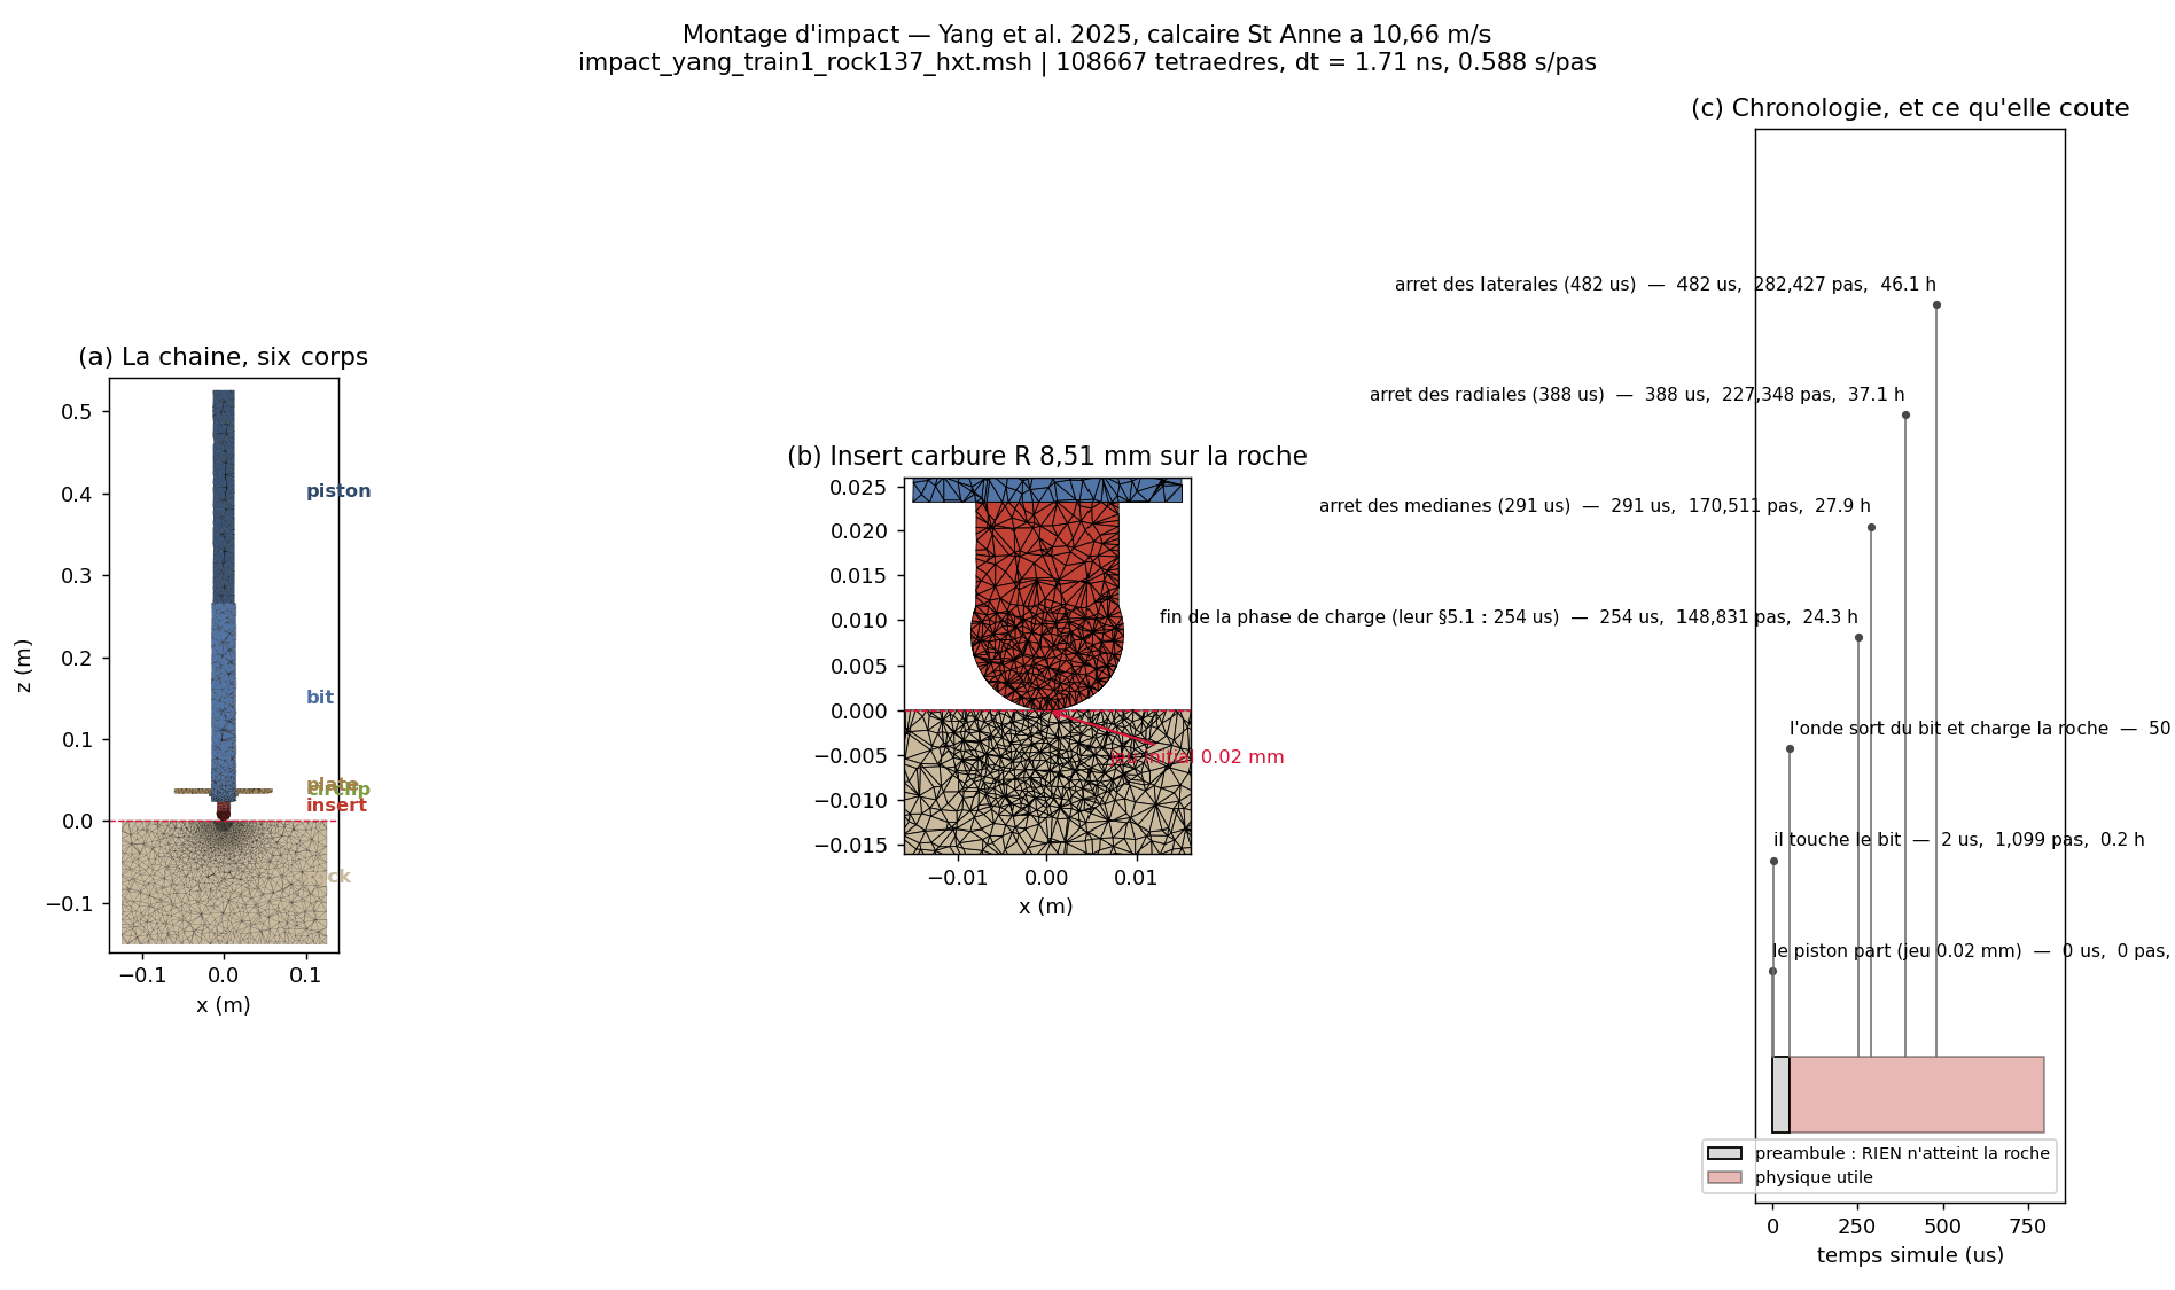
\includegraphics[width=\linewidth]{stanne_montage}
\caption{Montage de la réplique St Anne : chaîne de six corps, insert en carbure de rayon $8{,}51$~mm posé à $0{,}02$~mm de la roche, et coût en temps de calcul des événements de la chronologie (\cle{results/fig/config_stanne/}).}
\label{fig-montage}
\end{figure}

\subsection{Procédure}

Le guide d'utilisation fixe une procédure en cinq étapes, chacune issue d'un calcul perdu (\cle{GUIDE_rockim.md}, §4). La fenêtre de temps se dimensionne avant d'écrire la configuration : temps de vol $t_0 = \text{jeu}/v$, durée de contact de Hertz $t_c \approx 2{,}87\,(m^2/(R E^{*2} v))^{1/5}$, puis une marge ; un calcul mal dimensionné a tourné 4~h sans que rien n'atteigne la roche. La faisabilité de la rupture se vérifie ensuite par $2\,\Delta x < \ell_{cz} = E G_f/f_t^2 < a = \sqrt{R\delta}$ : avec $\ell_{cz} = 35$~mm pour un rayon de contact de $1{,}45$~mm, un calcul n'a rompu que 4 joints sur 158\,423. Un essai de fumée précède tout calcul de plus de 30~min, avec quatre contrôles : instant du premier contact, au moins une rupture, résidu du bilan sous $1~\%$, coût extrapolé. Le calcul se lance enfin avec un nombre de fils choisi, un seul fil donnant des sorties identiques au bit au calcul série (\cref{sec-fils}).

\subsection{Le banc Kuru, configuration v3-P}

La configuration de référence de l'impact sur granite de Kuru est \cle{configs/yang2026_bench_s25_v3P.cfg}. Elle dérive de \cle{yang2026_bench_s25.cfg}, que l'auteur du code a cessé de tenir pour référence : cette dernière combine la branche de décharge \cle{origin} et la naissance de contact calée, et le garde-fou d'énergie l'arrête à $2{,}9~\mu$s ; avec une rampe de naissance, elle crée $4{,}3$~J et s'arrête à $81~\mu$s (\cle{docs/RAPPORT_nuit_2026-09-13.md}, l.~60-85). La variante v3-P diffère par cinq options : branche \cle{plastic} avec cliquet sur les sécantes, contrainte normale lue sur la branche parabolique, pulvérisation limitée à la roche, raideur de contact prise sur le plus petit module, naissance de contact en rampe ; sa durée est de $200~\mu$s. Le \cref{tab-kuru} la détaille bloc par bloc.

\begin{table}[htbp]
\centering
\caption{Configuration v3-P du banc Kuru, bloc par bloc.}
\label{tab-kuru}
\begin{tabularx}{\linewidth}{@{}l X@{}}
\toprule
bloc & contenu \\
\midrule
géométrie & six corps ; roche cylindrique de rayon 125~mm et hauteur 150~mm ; insert hémisphérique de rayon $8{,}51$~mm ; bit de 30~mm de diamètre et 265~mm de long ; piston de $26{,}5$~mm et 260~mm ; jeux de $0{,}02$~mm ; maillage de résolution $s = 2{,}5$, soit 10\,563 tétraèdres \\
roche & granite de Kuru (table~1 de Yang et al. 2026) : $\rho = 2\,626$~kg/m$^3$, $E = 60$~GPa, $\nu = 0{,}24$, $f_t = 10{,}98$~MPa, $c = 29{,}84$~MPa, $\tan\varphi = 1{,}85$, $G_I = 50$~J/m$^2$, $G_{II} = 20\,G_I$ \\
métaux & acier $7\,850$~kg/m$^3$, 200~GPa ; carbure $15\,250$~kg/m$^3$, 600~GPa ; résistances portées à $10^{12}$~Pa, corps continus ; insert et circlip brasés au bit \\
joints & intrinsèques, pénalité 20, branche parabolique, adoucissement de Munjiza, enveloppe de Yang, plage de Coulomb, décharge \cle{plastic} avec cliquet, mort sur endommagement, sans amortisseur, quadrature aux milieux d'arêtes, règle des deux points sur trois \\
volume & co-rotationnel ; pulvérisation de Yang limitée à la roche ($\delta_0 = 0{,}014$~mm, $\delta_F = 0{,}4$~mm, $D_\text{max} = 0{,}9$) ; effet de vitesse continu, exposant $0{,}17$ en traction \\
contact & potentiel de Munjiza, raideur sur le plus petit module, activation adaptative, naissance en rampe, $\mu = 0{,}18$ pour la roche, couplage endommagement-contact \\
numérique & sans amortissement de Cundall ; \cle{dtFactor} $0{,}15$ ; pesanteur comptée dans le bilan ; arrêt si le résidu du bilan dépasse $2~\%$ \\
chargement & piston lancé à 9~m/s vers le bas \\
mesures & cinématique du bit, du piston et de l'insert ; jauge de contrainte à mi-bit \\
\bottomrule
\end{tabularx}
\end{table}

Le maillage de cette configuration est grossier : la référence de Yang et al. compte 230\,788 tétraèdres, le jumeau le plus fin de rockim ($s = 1$) 120\,185, et le cœur sous l'insert de ce jumeau est maillé à $1{,}37$~mm au lieu du millimètre annoncé. Le jumeau $s = 2{,}5$ n'est pas une étude de résolution du jumeau fin : son piston pèse $0{,}777$~kg contre $1{,}057$~kg, soit $31{,}5$~J d'énergie incidente contre $42{,}8$~J.

\subsection{Résultats connus du banc Kuru}

Le pas de temps vaut $2{,}83$~ns, soit 70\,733 pas pour $200~\mu$s. Le piston touche le bit à $2~\mu$s, l'onde passe à mi-bit vers $15~\mu$s et la jauge y lit une compression maximale de $173{,}0$~MPa, pour $178{,}3$~MPa par la théorie de l'impact unidimensionnel et environ 160~MPa chez Yang et al. L'enfoncement de l'insert progresse à $6{,}01$~m/s (pente entre 10 et $90~\%$) pour $5{,}62$~m/s chez Yang et al. L'enfoncement atteint $0{,}83$~mm, 294 joints rompent, dont $45~\%$ en traction, et 124 fragments se forment. Sur $100~\mu$s, le pic de la force de contact insert-roche vaut 11\,400~N et l'impulsion $0{,}264$~N\,s.

Deux grandeurs restent inexploitables sur ce banc. Le rebond n'est pas mesurable : aucun des 44 calculs d'impact archivés n'enregistre le retournement du bit, et la variante plastique prolongée à $300~\mu$s donne environ 1~m/s contre $4{,}65$~m/s chez Yang et al. La force de freinage n'est pas réconciliée : la force mesurée directement dans le contact insert-roche plafonne à $11{,}4$~kN sur $100~\mu$s, alors que l'estimateur cinématique du train rigide en déduit un pic de 55 à 65~kN, et ce même estimateur surestime le pic de $90~\%$ sur St Anne tout en reproduisant l'impulsion à $3{,}4~\%$ près (\cref{fig-stanne-fp}). Les comparaisons de force antérieures sont à refaire sur la force de contact mesurée.

\subsection{Sorties à exploiter}

Les colonnes \cle{grpZ}, \cle{grpVz} et \cle{grpFz} de \cle{history.csv} donnent la position, la vitesse et la force de contact nette de chaque corps suivi. La clé \cle{contactForcePairs} ajoute la force de contact exercée par un corps sur un autre, paire par paire, sommée en série et donc indépendante du nombre de fils ; la somme sur tous les partenaires du bit retrouve sa force nette à 0~N près. Cette mesure a révélé un piège : la plaque de guidage porte jusqu'à 3\,214~N sur le bit pendant les $30$ premières microsecondes, force que l'estimateur cinématique attribue à la roche. Les scripts de dépouillement sont listés en \cref{sec-annexe-reproduire}.

\section{Vérification}
\label{sec-verification}

\subsection{Cadre}

La campagne en cours adopte les définitions de la norme ASME V\&V~10~\cite{asme2019vv10} et d'Oberkampf et Roy~\cite{oberkampf2010vv}. La vérification établit que le code résout correctement ses équations, contre une solution analytique, une propriété mathématique ou une implémentation indépendante, sans donnée expérimentale. La validation établit que les équations représentent la roche, contre un essai qui n'a pas servi au calage. Un test de non-régression, dont la référence est une sortie antérieure de rockim, ne relève d'aucune des deux : il garantit que le code n'a pas changé, pas qu'il est juste (\cle{docs/VV_campagne.md}, l.~43-56). Cette section rassemble ce qui relève de la vérification ; la validation fait l'objet de la \cref{sec-validation}.

Les chiffres de cette section sont de deux natures. Les uns sont écrits dans les documents du dépôt. Les autres ont été rejoués le 6 octobre 2026 pour ce rapport, sur un exécutable compilé sous Linux à partir du commit \cle{f0209ef}, à un fil ; ils sont signalés comme tels.

\subsection{La suite de non-régression}

Le script \cle{tools/verify_suite.py} lance l'exécutable sur une configuration ou une sous-commande d'auto-test, lit les grandeurs imprimées et les compare à des références par une tolérance absolue propre à chaque contrôle. Il connaît aussi des contrôles qualitatifs : présence du verdict interne de l'auto-test, travail d'un amortisseur négatif ou nul, absence d'un déclenchement. Les références sont figées sur une base Linux du 11 août 2026, et un fichier de références par plateforme existe pour macOS ARM, car les tirages aléatoires de Voronoï et de Weibull diffèrent d'une bibliothèque standard à l'autre à graine égale.

La suite compte 118 tests, comptés en exécutant sa définition : 51 au niveau rapide, 56 de plus au niveau complet, 11 de plus au niveau exhaustif. Plusieurs documents en donnent un autre nombre (12, 44, 48 ou 104) : ces nombres sont datés et périmés, la suite ayant grossi par addition.

Le document de campagne classe ces 118 tests selon la nature de leur référence (\cref{tab-classement}). Seuls les 56 tests des quatre premières catégories relèvent de la vérification. Les 24 tests qui comparent un pic à $f_t$ figent l'écart mesuré un jour donné, de sorte qu'un écart de $1{,}4~\%$ ou de $15~\%$ passerait de la même façon s'il avait été enregistré tel quel. Les 38 tests de régression ne démontrent pas la justesse. Ce classement est déclaré dans le document ; la liste nominative test par test n'est pas outillée.

\begin{table}[htbp]
\centering
\caption{Classement des 118 tests de la suite selon la nature de leur référence (\cle{docs/VV_campagne.md}, Partie I §2).}
\label{tab-classement}
\begin{tabularx}{\linewidth}{@{}X r X@{}}
\toprule
catégorie & tests & référence \\
\midrule
analytique au point matériel ou sans maillage & 11 & formule exacte, VUMAT Fortran, conservation à deux corps \\
analytique sur une structure & 8 & barre en traction, allongement et réaction exacts \\
invariant au repos & 26 & aucune rupture, aucune injection sous charge nulle \\
invariant d'équivalence & 11 & deux réglages qui doivent coïncider, ou un poste qui ferme le bilan \\
pic contre $f_t$, écart figé & 24 & écart à $f_t$ mesuré un jour donné \\
régression pure & 38 & sorties antérieures de rockim \\
\bottomrule
\end{tabularx}
\end{table}

Rejouée pour ce rapport au niveau rapide, la suite passe 50 tests sur 51 en 19,5~min. Le seul échec, \cle{t1_toolcontact_penalty}, porte sur le banc de raclage en pénalité, cas construit pour pomper de l'énergie et déclaré chaotique : il donne un rapport d'injection de $2{,}985$ pour $4{,}426$ attendu, écart déjà consigné pour Linux dans le journal des modifications. La suite doit être lancée depuis la racine du dépôt, faute de quoi des chemins de maillage relatifs ne sont pas trouvés. Sous macOS ARM, le document de campagne déclare 39 tests sur 50, les 11 échecs étant tous des pics à écart figé ou des régressions dont les grandeurs post-pic sont déplacées par l'arithmétique flottante ; aucun test de vérification n'y échoue.

\subsection{Auto-tests}
\label{sec-selftests}

Douze sous-commandes \cle{rockim selftest-*} vérifient une brique sans maillage ou sur un maillage minimal ; huit sont branchées dans la suite. Le \cref{tab-selftests} donne leurs résultats rejoués.

\begin{table}[htbp]
\centering
\caption{Auto-tests rejoués le 6 octobre 2026 sous Linux, à un fil.}
\label{tab-selftests}
\begin{tabularx}{\linewidth}{@{}l X X@{}}
\toprule
auto-test & ce qui est vérifié & résultat rejoué \\
\midrule
\cle{potential2d} & collision élastique sans frottement par le potentiel de Munjiza 2D, frontale et oblique & $\Delta E_c/E_{c0} = 3{,}72\times10^{-12}$ et $5{,}12\times10^{-7}$ ; quantité de mouvement à $4{,}9\times10^{-15}$ \\
\cle{potential3d} & même essai entre tétraèdres & $2{,}05\times10^{-8}$ et $7{,}3\times10^{-9}$ ; quantité de mouvement à $4{,}7\times10^{-15}$ \\
\cle{potvolume3d} & même essai, force par volume de recouvrement & $7{,}1\times10^{-15}$ et $1{,}21\times10^{-11}$ \\
\cle{toolcontact} & algèbre du contact d'outil en vitesse ; chaîne de $N$ masses frappée à 10~m/s & écart relatif maximal $0{,}00996$ ; $N = 400$ : sortie à $19{,}936$~m/s pour 20, perte $0{,}2475~\% \approx 1/N$ \\
\cle{mc} & plateaux plastiques de Mohr-Coulomb contre $\sigma_c = 2c\cos\varphi/(1-\sin\varphi)$ & compression $-3{,}0\times10^{-9}~\%$ ; triaxial au plus $2{,}1\times10^{-9}~\%$ ; traction $-0{,}126~\%$ \\
\cle{pdc3d} & géométrie du couteau PDC chanfreiné, avec variantes qui doivent échouer & 14 contrôles passés, aucun échec \\
\cle{saksala2011}, \cle{dpdfh} & lois au point matériel & s'exécutent ; la comparaison au Fortran n'est pas faite par la sous-commande \\
\bottomrule
\end{tabularx}
\end{table}

Les écarts de $8\times10^{-14}$ et $4{,}7\times10^{-12}$ annoncés pour les portages des VUMAT de Saksala et du DP-DFH ne sont pas rejouables depuis le dépôt seul : la sous-commande écrit la trajectoire de contrainte, et la référence Fortran n'est pas dans le dépôt. Quatre autres auto-tests (empreinte triaxiale, endommagement plastique, fissure fixe, DFH reformulé) ne sont pas dans la suite et n'ont pas été rejoués. En pénalité, le même nœud au repos repart en un pas à 373~m/s, soit $18{,}7$ fois la borne physique $2v$, et un amortissement de Cundall de $0{,}05$ fait perdre $14{,}7~\%$ de la vitesse de sortie à la chaîne de masses.

\subsection{Bilan d'énergie}
\label{sec-B4}

Le bilan d'énergie, ajouté le 14 août 2026 en FDEM 2D et 3D, applique le théorème de l'énergie cinétique aux nœuds : la variation d'énergie cinétique égale la somme des travaux des familles de forces, plus un résidu (\cle{DOCUMENTATION_rockim.md}, l.~2622-2641). Les postes sont les éléments, les joints, les amortisseurs, le contact général et son frottement, l'amortissement de Cundall, les frontières, l'outil, les platines, les forces de volume et un poste d'intégration. Ce dernier corrige exactement l'écart du saute-mouton, $f^2\Delta t^2/(2m)$ par nœud et par pas, entre les compteurs qui lisent la vitesse d'avant le pas et le théorème discret qui veut la moyenne : sans lui, le résidu de la percussion 2D valait $91~\%$, avec lui $0{,}017~\%$. Le bilan est déclaré bon quand le résidu reste sous $1~\%$ du flux brut échangé.

Les résidus mesurés sont de l'ordre de l'arrondi en élastique et petits sur les impacts. Une barre en traction rejouée pour ce rapport donne $-5{,}6\times10^{-17}$~J en FDEM 3D et $3{,}4\times10^{-17}$~J en éléments finis 3D. La documentation donne $0{,}017~\%$ sur la percussion 2D, $0{,}005~\%$ sur la percussion 3D et $-5\times10^{-24}$~J à charge nulle entre deux corps ; le calcul St Anne de $300~\mu$s ferme à $1{,}5\times10^{-7}~\%$.

Le bilan est une identité comptable et ne voit pas une création d'énergie logée dans un poste compté. La coupe PDC 2D du 18 août injectait 408 fois le travail de l'outil pendant que le bilan affichait un résidu de $1{,}9\times10^{-10}~\%$. Pour cette raison, des indicateurs dédiés s'ajoutent au bilan pour le contact d'outil (rapport d'injection, borne $2v$), et la loi de joint se juge sur cycle fermé (\cref{sec-decharge}). Le garde-fou \cle{budgetAbortPct} arrête un calcul dont le résidu dépasse un seuil ; sans compter la pesanteur dans le bilan (\cle{energyBodyForces = on}), il coupait à tort un calcul sain sur un résidu de $175~\%$ qui était le travail de la pesanteur.

Le bilan a une réserve d'instrumentation en FDEM 3D : le poste des éléments est unique, exact en élastique et approché sous loi de volume ou plafond, et la dissipation plastique du volume n'est pas séparée (\cle{AUDIT_loi_adaptative_2026-09-11.md}, §5).

\subsection{Contrôles à charge nulle}

Un contrôle à charge nulle laisse un modèle au repos, ou sous une vitesse de $10^{-12}$~m/s, et exige zéro joint rompu et un travail d'amortisseur négatif ou nul. La suite en compte 26, en 2D et en 3D, un par option de loi ou de contact ajoutée. Ils ont attrapé de vrais défauts : 158 joints rompus à charge nulle sur un maillage de Delaunay avant correction, et 5 joints rompus par des tétraèdres exactement tangents dans le contact par potentiel 3D. Tous ceux du niveau rapide passent, rejoués pour ce rapport.

\subsection{Nombre de fils et déterminisme}
\label{sec-fils}

Les résultats dépendent du nombre de fils. À un fil, les sorties sont identiques au bit à celles du calcul série ; à nombre de fils fixé, elles sont déterministes ; entre deux nombres de fils, l'ordre des sommes change et les pics s'écartent. La documentation annonce environ $2~\%$ ; le cas mesuré le plus documenté donne 7\,916,75~N à 4 fils contre 7\,791,04~N à 2 fils, soit $1{,}6~\%$ (\cle{tools/BITID.md}). Le banc de raclage en pénalité rompt 8 joints au lieu de 2 hors d'un fil. La suite se certifie donc à un fil.

L'identité au bit sert à montrer qu'une option nouvelle ne change rien quand elle est absente. Huit configurations courtes, ancrées à 4 fils le 5 septembre 2026, voient l'empreinte de leurs sorties comparée à chaque modification (\cle{tools/bitid.py}) ; toute ancre changée exige une ligne au journal des modifications. Cette discipline protège contre le changement involontaire ; elle ne prouve pas la justesse.

\subsection{Comparaisons à un autre code et à Hertz}

Une comparaison à Abaqus avec la loi de Saksala sur le même maillage, une sphère à 8~m/s, a été faite le 31 juillet avec des critères fixés avant calcul : pic filtré $+7{,}9~\%$, énergie $+0{,}9~\%$, pénétration $+1{,}1~\%$, restitution $0{,}111$ contre $0{,}059$. Une seconde comparaison avec une loi d'endommagement plastique est passée de $-20~\%$ à $+2{,}8~\%$ après l'ajout de quatre clés choisies pour se rapprocher d'Abaqus, ce que le document qualifie d'ajustement et non de vérification. Les fichiers de ces comparaisons ne sont pas dans le dépôt. La figure \cle{figures_impact/compare_fdelta_abaqus_rockim.png} compare le bruit de deux cas différents et non leurs résultats.

La réponse en force d'un impact élastique a été confrontée à Hertz sur quatre maillages (\cref{fig-hertz}). La réponse globale suit Hertz à $-25~\%$ à $+30~\%$ près en fin de charge, sans converger vers le rapport 1 au raffinement, et le pic local de contrainte n'est pas résolu : il passe de 266 à 2\,931~MPa quand la taille d'élément passe de $4{,}74$ à $0{,}80$~mm, pour une pression de Hertz de 4\,114~MPa. Le document de campagne écrit pourtant que le contact n'a pas de référence analytique en force ; le banc de la sphère sur un plan, préparé, reprend cette question avec des critères écrits (\cref{sec-validation}).

\begin{figure}[htbp]
\centering
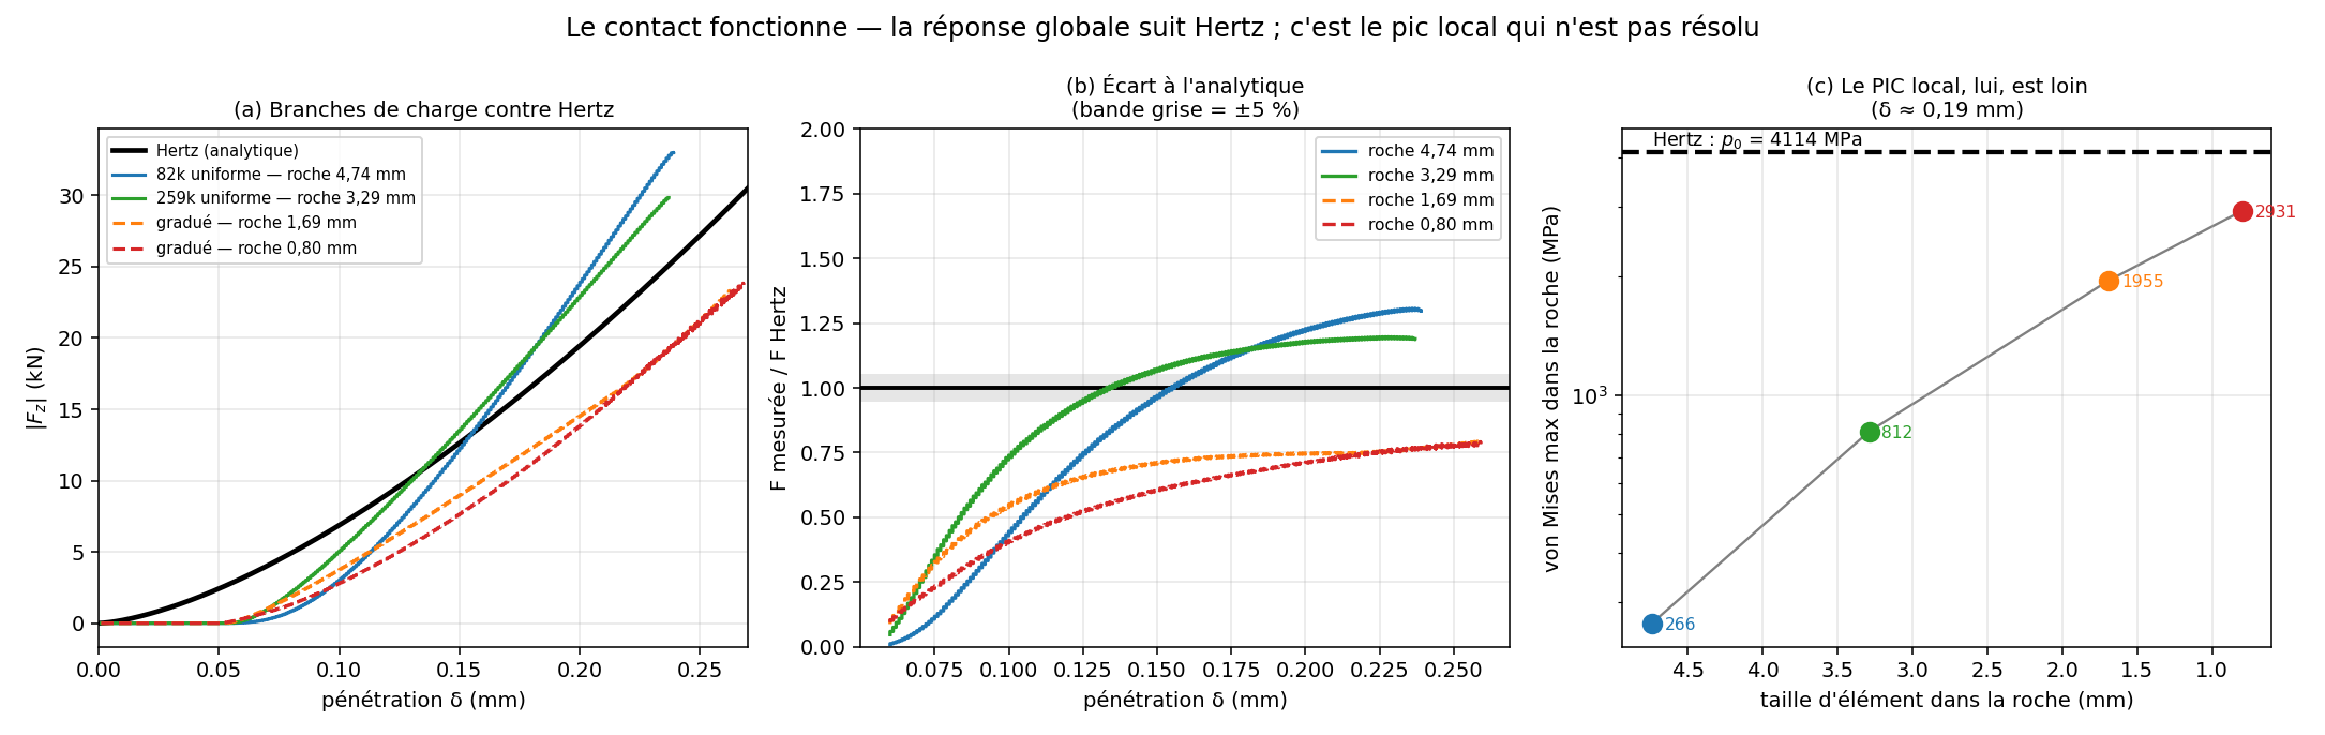
\includegraphics[width=\linewidth]{hertz_compare}
\caption{Impact élastique d'une sphère sur quatre maillages de roche : force contre enfoncement, rapport à Hertz et pic de von Mises contre taille d'élément (\cle{figures_impact/plot_hertz.py}).}
\label{fig-hertz}
\end{figure}

\subsection{Audits}

Quatre audits ont précédé la campagne de vérification. La revue de fiabilité 3D du 14 août a établi un plan à critères de réfutation après l'instabilité de $2{,}4$~MJ, dont le garde-fou d'énergie ; le cas explosif n'a jamais été rejoué depuis les correctifs. L'audit de la loi adaptative du 11 septembre a confronté la loi codée à une note de loi constitutive : 2 briques conformes, 11 partielles, aucune absente, et six mécanismes dissipatifs parasites armés par défaut. L'audit du 13 septembre, conduit par quatre agents en lecture seule, a relevé la pénalité de contact absente du budget du pas, la contrainte normale divisée par deux sous la branche parabolique et le contact roche-roche dix fois trop raide ; les corrections sont des options désactivées par défaut. Le plan de robustesse du 5 septembre a diagnostiqué un mode de panne dominant, le défaut silencieux, et a conduit au refus des clés inconnues et à l'ancre d'identité au bit ; les références Linux et Windows de la suite et l'intégration continue qu'il prévoyait ne sont pas faites.

\section{Validation}
\label{sec-validation}

\subsection{Démarche de la campagne}

La campagne de vérification et validation a commencé le 3 octobre 2026 (\cle{docs/VV_campagne.md}). Elle reprend la démarche en deux temps des codes FDEM publiés (Guo et Solidity, Lisjak et Y-Geo~\cite{lisjak2013thesis,mahabadi2012ygeo}, Fukuda, HOSS) : des cas à solution exacte d'abord, la reproduction d'articles ensuite. Elle s'en distingue par une règle : chaque critère d'acceptation est chiffré et écrit avant le premier calcul, et un échec est consigné tel quel, sans retouche du critère. La partie II du document porte les cas à solution exacte (bancs P1 à P5), la partie III la reproduction chiffrée d'articles (B1 à B9), la partie IV un calage unique sur le Red Bohus (compression simple, brésilien, triaxial à 20 et 50~MPa) suivi d'une prédiction sans retouche du triaxial à 75 et 100~MPa.

Chaque banc vit dans un dossier de \cle{vv/} avec un script qui prépare, lance et analyse les calculs, ses critères en constantes, un fichier de résultats et ses figures. Un lanceur répartit les calculs sur les cœurs et reprend les calculs interrompus. Les résultats de la campagne ont été produits sous macOS ARM.

Au 6 octobre 2026, deux bancs ont tourné en campagne (\cref{tab-bancs}). Sept autres sont préparés avec leurs critères et n'ont tourné qu'en essai de fumée, sur maillage grossier ou durée réduite ; leurs chiffres valident la chaîne de calcul, pas le résultat. Les parties III et IV sont vides.

\begin{table}[htbp]
\centering
\caption{Statut des bancs de la campagne de vérification et validation au 6 octobre 2026.}
\label{tab-bancs}
\begin{tabularx}{\linewidth}{@{}l X l X@{}}
\toprule
banc & référence & statut & verdict \\
\midrule
P1.1 onde dans une barre & d'Alembert & exécuté & \cle{fem3d} passe ; FDEM adaptatif échoue au seul bilan ; intrinsèque $p_f = 20$ échoue \\
P2.1 bloc glissant & $L = v_0^2/(2\mu g)$ & exécuté & potentiel passe ; pénalité échoue \\
P1.2, P1.3 élasticité & Kirsch, champ homogène & fumée & aucun \\
P2.2 sphère sur un plan & Hertz & fumée & aucun \\
P3.1 fissure pressurisée & mécanique de la rupture, Guo & fumée & aucun \\
P3.3 fissure en aile & Lisjak, Y-Geo & fumée & aucun \\
P4.1, P4.2 flexion, brésilien & poutre, Hondros, Guo & essai à blanc & aucun \\
B4 à B7 articles & AbuAisha, Wang, Yan, Yang & B6 relancé & B6 : reproduction en échec \\
B8, B9 impact et coupe & Saksala, Heilman, LeBaron & fumée & aucun \\
P3.2 énergie de fissure & $G_f$ fois l'aire rompue & non préparé & aucun \\
\bottomrule
\end{tabularx}
\end{table}

\subsection{Onde de compression dans une barre}
\label{sec-V1}

Ce banc vérifie la célérité, l'impédance et les réflexions, et mesure un ordre de convergence : une erreur à ce niveau se retrouverait dans tous les bancs d'impact. La barre mesure $8 \times 8 \times 400$~mm, avec $\rho = 2\,650$~kg/m$^3$, $E = 60$~GPa et $\nu = 0{,}25$ ; ses quatre faces latérales sont sur rouleaux, ce qui rend le problème exactement unidimensionnel, sans la dispersion de Pochhammer, avec $c = \sqrt{M/\rho} = 5\,212{,}47$~m/s. Une vitesse de $0{,}1$~m/s en trapèze de 4, 12 et $4~\mu$s est imposée à une extrémité, l'autre est libre, et le calcul dure $250~\mu$s, soit $1{,}6$ aller-retour. La solution exacte est la série de d'Alembert avec réflexions ; le plateau de la réaction vaut $\rho c v_0 A = 88{,}40$~N. Les critères, fixés avant calcul sur le maillage le plus fin, sont une erreur $L^2$ du déplacement d'au plus $2~\%$, des erreurs de célérité et de force d'au plus 1 et $2~\%$, un résidu du bilan d'au plus $10^{-6}~\%$ et un ordre de convergence d'au moins 1.

\begin{table}[htbp]
\centering
\caption{Onde dans une barre : erreurs mesurées par variante et taille d'élément $h$.}
\label{tab-V1}
\small
\begin{tabular}{@{}lrrrrrr@{}}
\toprule
variante & $h$ (mm) & tétraèdres & $e_u$ & $c$ & $F$ & résidu du bilan \\
\midrule
\cle{fem3d} & 4 & 3\,688 & $0{,}46~\%$ & $-0{,}05~\%$ & $-0{,}04~\%$ & $2{,}6\times10^{-12}~\%$ \\
\cle{fem3d} & 1 & 125\,486 & $0{,}05~\%$ & $<0{,}01~\%$ & $<0{,}01~\%$ & $1{,}2\times10^{-10}~\%$ \\
FDEM adaptatif & 2 & 20\,435 & $0{,}17~\%$ & $+0{,}04~\%$ & $<0{,}01~\%$ & $5{,}5\times10^{-4}~\%$ \\
FDEM intrinsèque $p_f = 20$ & 4 & 3\,688 & $7{,}7~\%$ & $-2{,}9~\%$ & $-2{,}9~\%$ & $1{,}5\times10^{-3}~\%$ \\
FDEM intrinsèque $p_f = 20$ & 2 & 20\,435 & $8{,}6~\%$ & $-3{,}2~\%$ & $-3{,}3~\%$ & $3{,}5\times10^{-4}~\%$ \\
\bottomrule
\end{tabular}
\end{table}

Le solveur éléments finis passe les cinq critères (\cref{tab-V1}), avec un ordre observé de $1{,}58$ sur le déplacement (\cref{fig-V1conv}). L'ordre inférieur à 2 est attribué aux quatre angles du trapèze, qui limitent la régularité de la solution exacte. L'erreur $L^2$ sur la réaction décroît de $16~\%$ à $3{,}5~\%$ ; elle vient des oscillations de dispersion numérique au retour de l'onde, le plateau étant exact.

La FDEM en insertion adaptative reproduit les éléments finis à $10^{-4}$ près maillage par maillage, avec un ordre de $1{,}46$, mais échoue au critère du bilan : son résidu vaut $2{,}2\times10^{-3}$ à $5{,}5\times10^{-4}~\%$. Le document l'attribue au décalage d'un demi-pas entre les compteurs de travail et le saute-mouton, résidu d'ordre $\Delta t$ qui décroît avec le pas, et non à une création d'énergie. Le critère, calibré sur les éléments finis, est jugé inadapté mais n'a pas été changé après coup.

\begin{figure}[htbp]
\centering
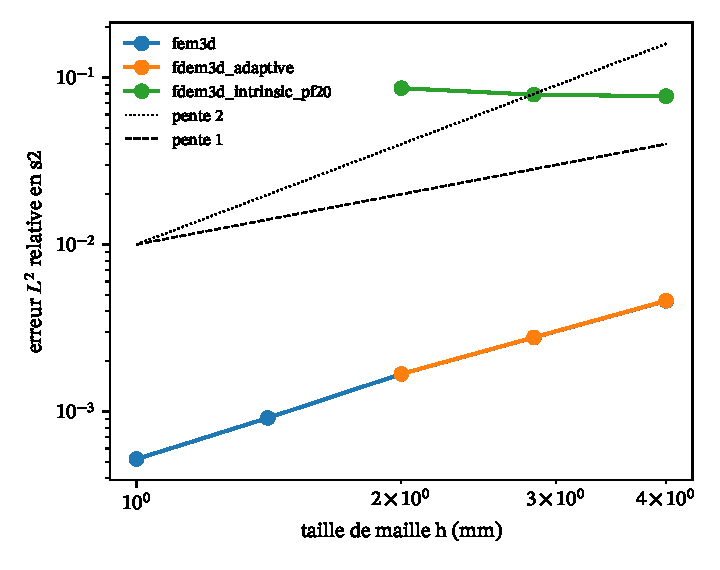
\includegraphics[width=0.62\linewidth]{fig_convergence}
\caption{Onde dans une barre : erreur $L^2$ du déplacement à mi-longueur contre la taille d'élément, pour les éléments finis, la FDEM adaptative et la FDEM intrinsèque à $p_f = 20$.}
\label{fig-V1conv}
\end{figure}

La FDEM en insertion intrinsèque à $p_f = 20$, réglage du banc d'impact, échoue : l'onde est $2{,}9$ à $3{,}2~\%$ trop lente et le plateau de force trop faible d'autant, sans aucune rupture, et l'erreur ne décroît pas avec $h$ (ordre $-0{,}16$), parce que le nombre de joints par unité de longueur croît comme $1/h$. Avec ce réglage, les ondes d'un impact arrivent environ $3~\%$ en retard et la force de contact initiale est sous-estimée d'environ $3~\%$, indépendamment du maillage.

Un balayage de la pénalité de 10 à 200 a testé un modèle de joints en série, $c_\text{eff}/c = (1 + \alpha/p_f)^{-1/2}$, avec $\alpha = 1{,}21$ calé sur le seul point $p_f = 20$ et écrit avant le balayage (\cref{fig-V1pen}). La prédiction tient à $0{,}05$ point près sur toute la plage ; l'ajustement sur les huit points donne $\alpha = 1{,}239$. Le retard vaut $-5{,}54~\%$ à $p_f = 10$, $-1{,}23~\%$ à 50, $-0{,}65~\%$ à 100 et $-0{,}35~\%$ à 200, ce dernier indépendant de $h$. Le pas de temps décroît comme $1/\sqrt{p_f}$. La règle qui en sort est $p_f \geq \alpha/(2\varepsilon) \approx 0{,}62/\varepsilon$ pour un biais de célérité $\varepsilon$ : 62 pour $1~\%$, 124 pour $0{,}5~\%$, au prix d'un pas plus petit d'un facteur $1{,}8$ ou $2{,}5$ par rapport à $p_f = 20$. Le banc de la fissure pressurisée en tient déjà compte avec $p_f = 100$.

\begin{figure}[htbp]
\centering
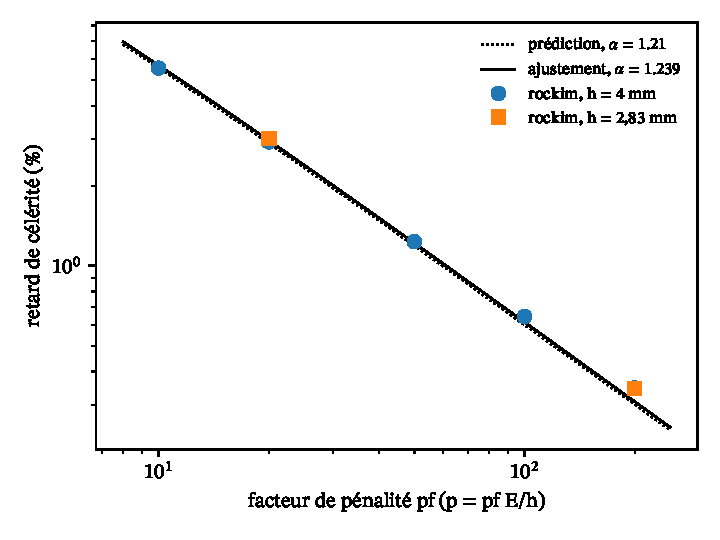
\includegraphics[width=0.62\linewidth]{fig_penalite}
\caption{Retard de célérité de l'onde contre le facteur de pénalité intrinsèque, mesuré sur deux maillages, avec la prédiction écrite avant le balayage et l'ajustement.}
\label{fig-V1pen}
\end{figure}

Le banc a trois réserves. La barre est confinée latéralement, la barre libre dispersive n'est pas couverte. Le pas de la FDEM est commandé par les tétraèdres aplatis (hauteur inscrite de $0{,}22$~mm à $h = 2$~mm), ce qui rend le calcul 40 à 100 fois plus coûteux qu'en éléments finis. Les résultats dépendent du générateur de maillage au-delà de la quatrième décimale.

\subsection{Bloc glissant jusqu'à l'arrêt}
\label{sec-P21}

Ce banc vérifie le frottement de Coulomb du contact général, d'après Xiang et al. 2009, repris en 3D par Fukuda et al. Un cube de 50~mm ($E = 1$~GPa) glisse sur une dalle fixe avec $\mu = 0{,}5$ sous la pesanteur ; les deux corps sont continus, leurs maillages ne coïncident pas, et seul le contact général les relie. Sans basculement, le bloc s'arrête à $L = v_0^2/(2\mu g)$. Les critères sont un écart d'au plus $2~\%$ sur la distance d'arrêt et sur la trajectoire.

\begin{table}[htbp]
\centering
\caption{Bloc glissant : distance d'arrêt simulée contre exacte selon la loi de contact et la vitesse initiale.}
\label{tab-P21}
\small
\begin{tabular}{@{}lrrrrl@{}}
\toprule
contact & $v_0$ (m/s) & $L$ simulé (mm) & $L$ exact (mm) & écart & verdict \\
\midrule
potentiel & $0{,}5$ & $25{,}93$ & $25{,}48$ & $+1{,}74~\%$ & passe \\
potentiel & 1 & $102{,}92$ & $101{,}94$ & $+0{,}96~\%$ & passe \\
potentiel & 2 & $410{,}27$ & $407{,}75$ & $+0{,}62~\%$ & passe \\
pénalité & $0{,}5$ & $-0{,}46$ & $25{,}48$ & $-102~\%$ & échoue \\
\bottomrule
\end{tabular}
\end{table}

Le contact par potentiel reproduit la cinématique aux trois vitesses (\cref{tab-P21,fig-P21}). Le bloc glisse un peu trop loin, d'autant moins que la vitesse est grande, ce que le document attribue à la régularisation du frottement à très faible vitesse en fin d'essai. Sur le premier millimètre, le travail de frottement égale $\mu m g$ fois la distance à $10^{-5}$ près. Le contact par pénalité, défaut de rockim, échoue : le bloc accroche par son arête les triangles de la dalle, bascule, son centre monte de $4{,}7$~mm, il retombe en arrière et finit $0{,}46$~mm derrière son point de départ, avec un bilan d'énergie pourtant fermé à $7\times10^{-12}~\%$. La règle qui en sort impose le contact par potentiel dès qu'un corps glisse sur un autre à travers des maillages non coïncidents ; les configurations d'impact l'appliquent déjà. Le basculement n'est jugé qu'indirectement : le critère de rotation déclaré dans le script n'est pas calculé.

\begin{figure}[htbp]
\centering
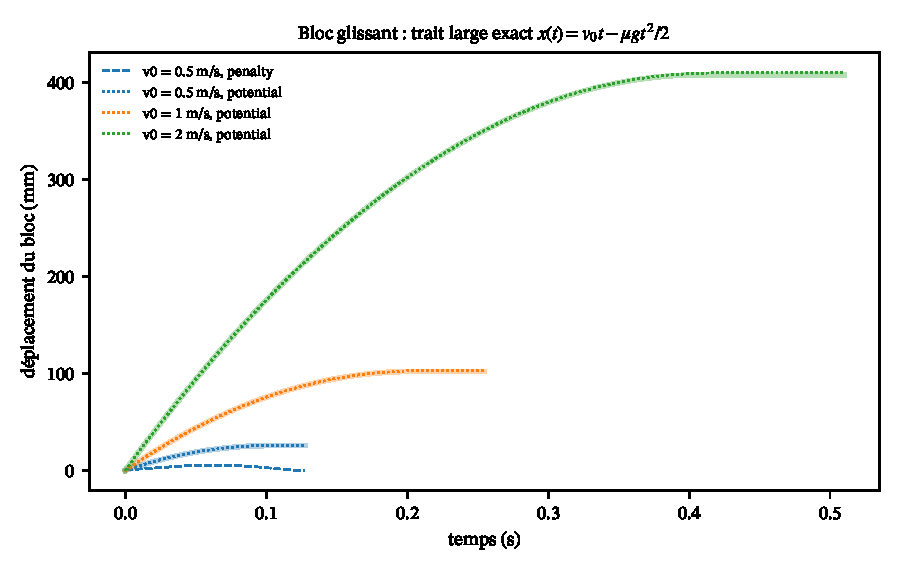
\includegraphics[width=0.62\linewidth]{fig_bloc}
\caption{Bloc glissant : déplacement contre temps pour trois vitesses initiales, contact par potentiel et par pénalité, comparé à la solution exacte en trait large.}
\label{fig-P21}
\end{figure}

\subsection{Bancs préparés}

Les bancs suivants ont leurs critères écrits et un essai de fumée ; aucun n'a de résultat de campagne. Le banc d'élasticité P1.2-P1.3 vérifie un champ homogène à la précision machine et la solution de Kirsch autour d'un trou ; l'essai de fumée passe le champ homogène à $7{,}5\times10^{-8}$. Le banc de la sphère sur un plan P2.2 compare le contact par potentiel à Hertz sur quatre raffinements ; l'essai court donne une force filtrée à $+4{,}6~\%$ et un enfoncement à $-3{,}6~\%$ de Hertz, le pic brut étant à $+36~\%$. Le banc de la fissure pressurisée P3.1 reprend le cas de Guo et doit quantifier l'objectivité de la rupture vis-à-vis du maillage, lacune ouverte du code ; la variante la plus fine est estimée à 71 à 114~h de calcul. Le banc de la fissure en aile P3.3 vise la contrainte d'amorçage de $7{,}0$~MPa et l'angle de $64^\circ$ de Lisjak ; deux des quatre formules analytiques de comparaison sont des reconstructions non vérifiées. Les bancs de flexion et de brésilien P4 reprennent Guo ; les critères écrits avant calcul annoncent qu'ils ne peuvent pas tous passer, parce que Guo trouve une résistance brésilienne de $0{,}65\,f_t$ alors qu'un modèle qui respecte Hondros doit amorcer au centre près de $f_t$. Le banc B8 compare le portage de la loi de Saksala à l'impact de bouton publié~\cite{saksala2011ijnamg} ; c'est une comparaison de code à code avec la même loi.

\subsection{Reproduction de Yang et al. 2025 : calcaire de St Anne}
\label{sec-stanne}

L'impact d'un insert sur le calcaire de St Anne à $10{,}66$~m/s~\cite{yang2025validation} est la comparaison la plus aboutie, et la seule menée sur un calcul complet de $300~\mu$s. Le maillage compte 108\,667 tétraèdres, dont un cœur de 14\,030 à $1{,}42$~mm d'arête médiane sous l'insert ; le matériau est celui de la table~4 de l'article ; la pénalité est prise sur les arêtes avec $p_0 = 3\,000$~GPa ; la loi de joint est \cle{plastic} avec plage de Coulomb et cliquet ; la pulvérisation et la viscosité sont désactivées. Le calcul a duré 29~h~21 sur 14 fils.

Les sept critères de l'article ne sont publiés que sous forme de graphiques et ont été lus à $10~\%$ près au mieux ; la chronologie vient du texte et est exacte (\cref{tab-stanne}). La contrainte au taillant, la vitesse d'indentation, le rayon du cratère et la fin de la phase de charge tombent à 6 à $12~\%$ de la simulation de Yang et al., de l'ordre de la dispersion expérimentale et du coefficient de variation de $10~\%$ annoncé par les auteurs. L'enfoncement et la masse de fragments s'écartent nettement, dans le même sens d'un cratère trop ouvert ; trois causes possibles ne sont pas départagées : le réglage du brossage des fragments, un cratère réellement plus ouvert, des éléments comptés qu'un brossage physique ne détacherait pas. La longueur des fissures radiales dépend d'une convention non tranchée, avec un facteur $1{,}7$ entre les deux définitions possibles. Le rebond n'est pas mesuré, car il faudrait au moins $450~\mu$s : la configuration à $500~\mu$s est prête mais n'a pas été lancée.

\begin{table}[htbp]
\centering
\caption{Réplique St Anne à $300~\mu$s : critères de Yang et al. 2025 lus sur les figures 9 et 10, et valeurs de rockim.}
\label{tab-stanne}
\small
\begin{tabular}{@{}lrrrr@{}}
\toprule
critère & Yang FDEM & Yang essai & rockim & écart \\
\midrule
contrainte au taillant & 200~MPa & 200~MPa & $212{,}3$~MPa & $+6~\%$ \\
vitesse d'indentation & $8{,}0$~m/s & $7{,}9$~m/s & $7{,}34$~m/s & $-8~\%$ \\
enfoncement maximal & $1{,}10$~mm & $1{,}05$~mm & $1{,}292$~mm & $+17~\%$ \\
vitesse de rebond & $5{,}6$~m/s & $4{,}2$~m/s & non mesurée & sans objet \\
longueur radiale & 32~mm & 31~mm & $29{,}6$ ou $17{,}7$~mm & $-8$ ou $-45~\%$ \\
rayon du cratère & $13{,}5$~mm & 13~mm & $12{,}00$~mm & $-11~\%$ \\
masse de fragments & $2{,}5$~g & $1{,}2$~g & $4{,}70$~g & $+88~\%$ \\
fin de la phase de charge & $254~\mu$s & non publiée & $284{,}3~\mu$s & $+12~\%$ \\
\bottomrule
\end{tabular}
\end{table}

Le bilan d'énergie du calcul ferme : l'énergie cinétique passe de $60{,}12$ à $3{,}28$~J, le résidu vaut $-9{,}8\times10^{-8}$~J, soit $1{,}5\times10^{-7}~\%$ de l'échelle, sur 12\,090 facettes rompues. La rupture dissipe $34{,}5$~J, le frottement $27{,}8$~J, les joints $14{,}5$~J, et $18{,}1$~J restent stockés en énergie élastique. Le réseau de fissures forme un noyau broyé sous l'insert et des branches radiales (\cref{fig-stanne-joints}) ; la partition entre traction et cisaillement des couleurs n'est qu'indicative, à cause de la normalisation retenue pour le mode de rupture.

\begin{figure}[htbp]
\centering
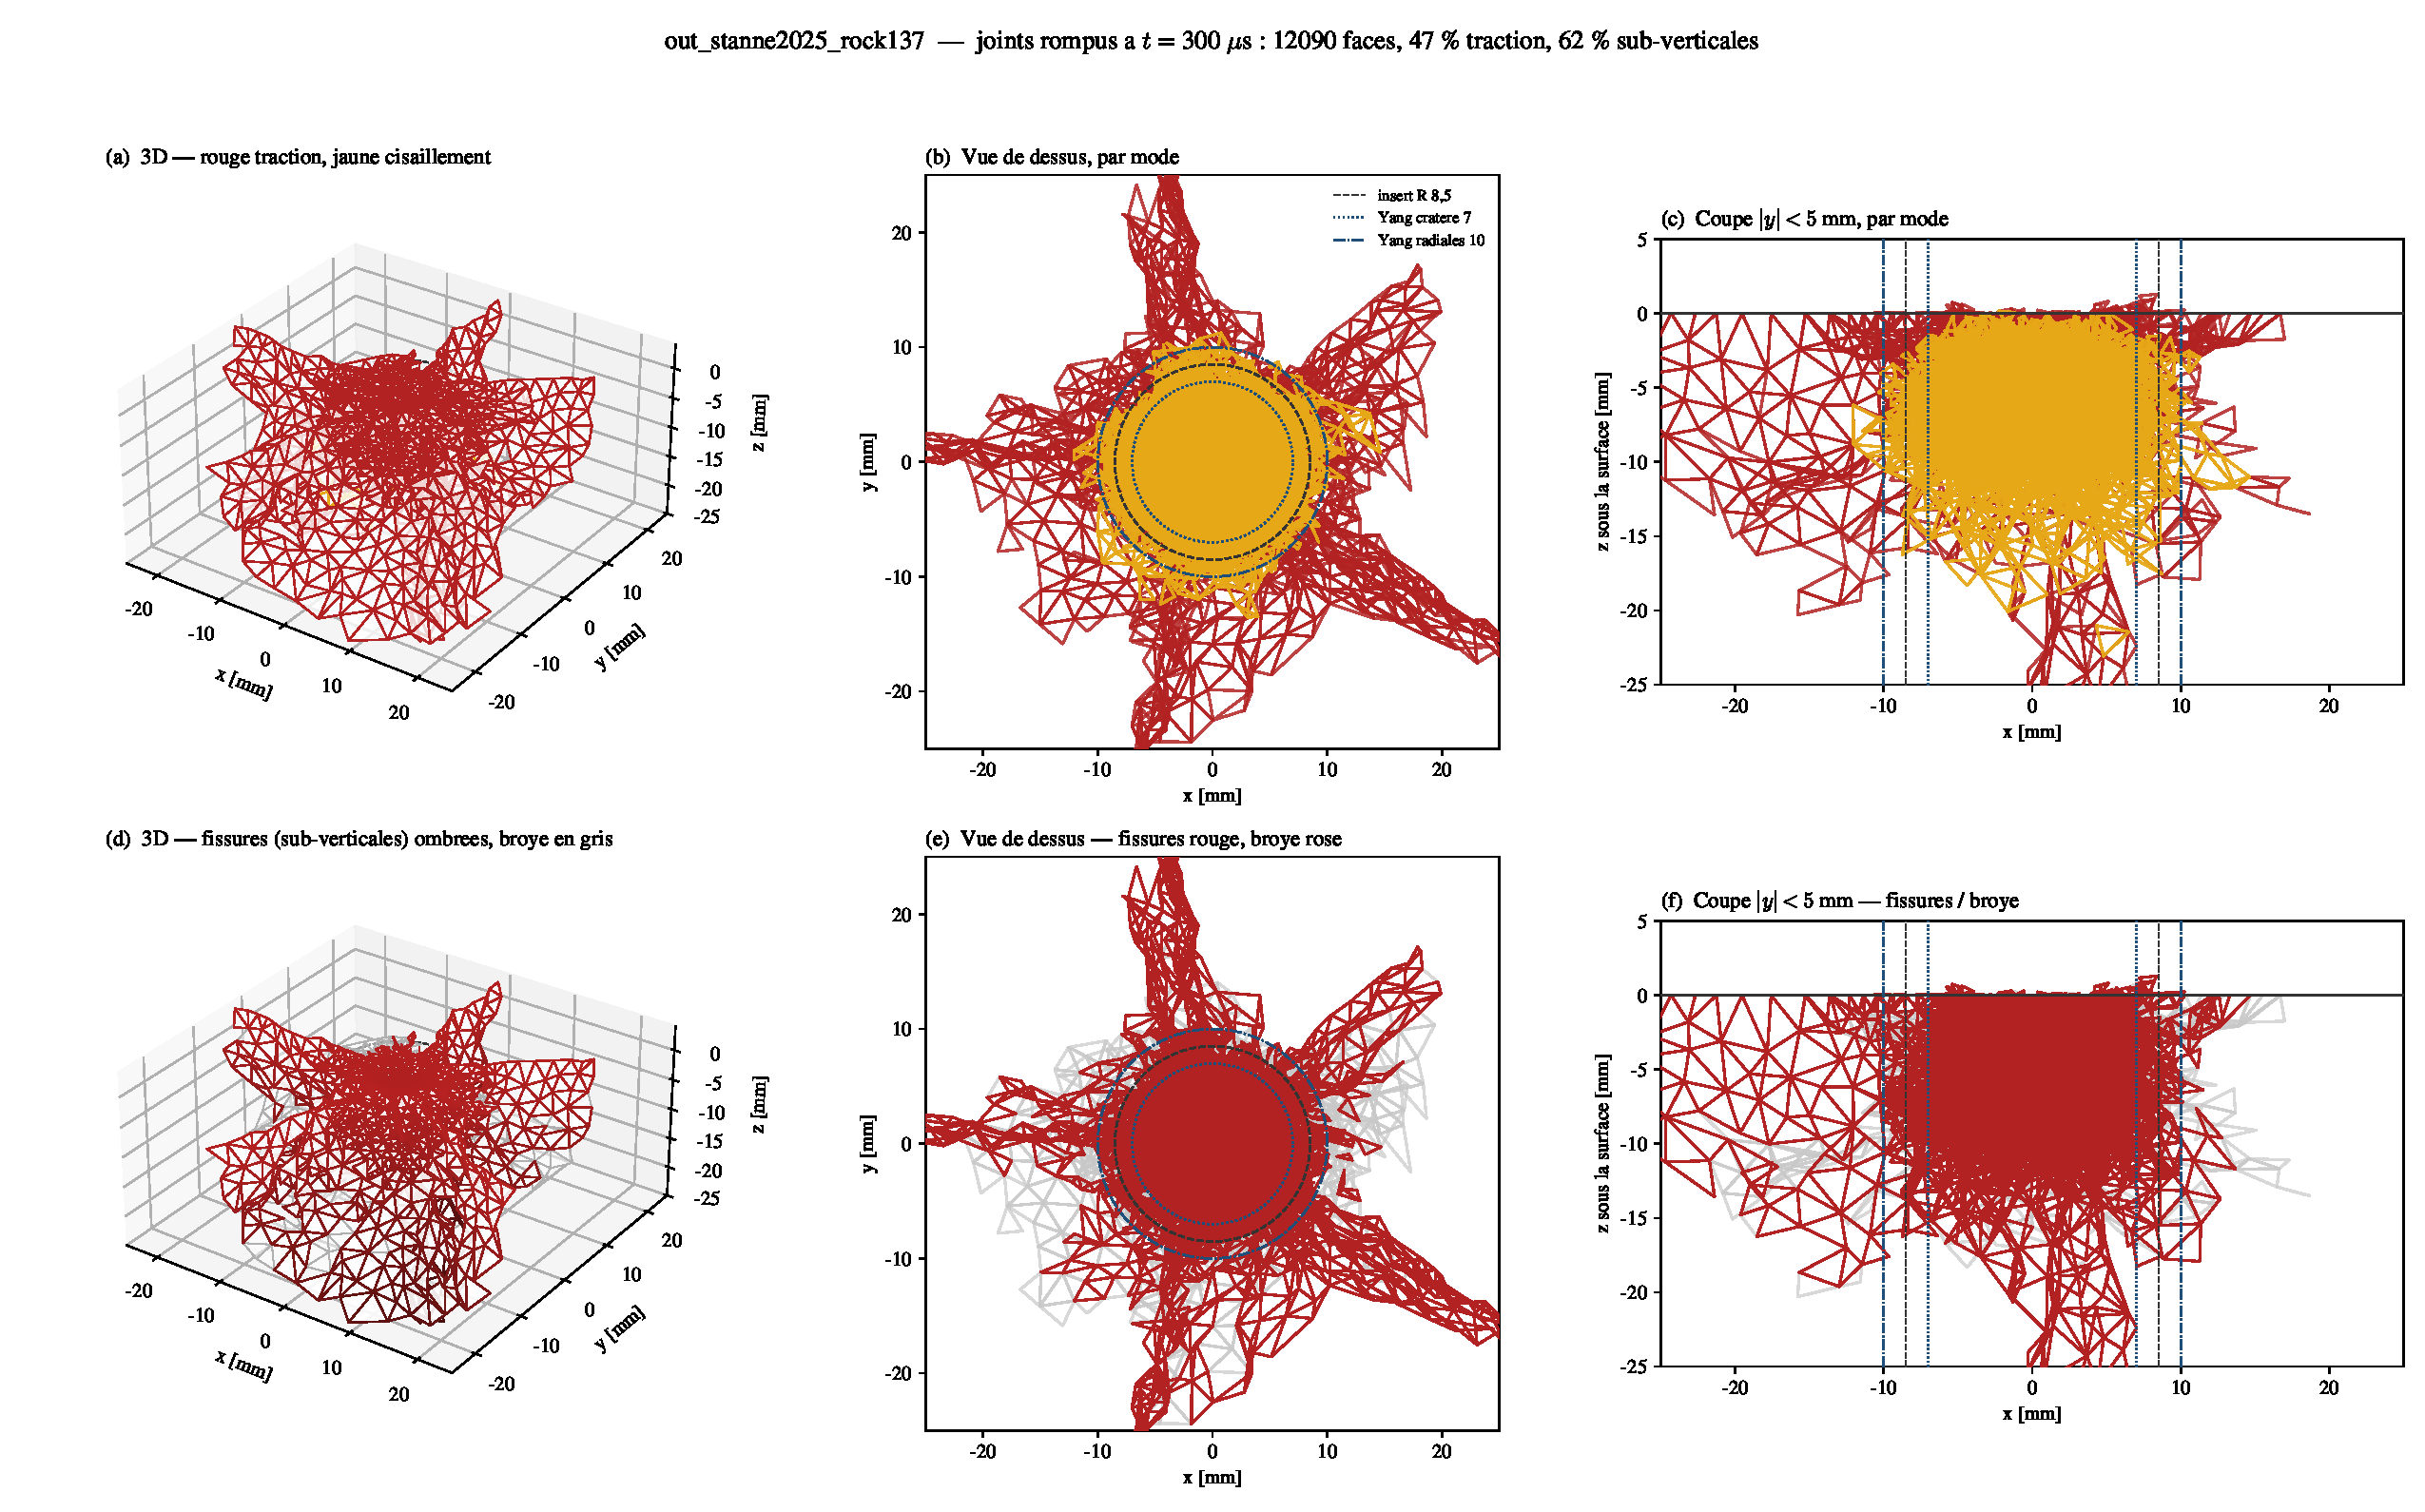
\includegraphics[width=\linewidth]{stanne_joints}
\caption{Réplique St Anne à $300~\mu$s : 12\,090 facettes rompues en vue 3D, de dessus et en coupe, colorées par mode de rupture (haut) et par type, fissure ou broyage (bas).}
\label{fig-stanne-joints}
\end{figure}

La force de contact mesurée entre l'insert et la roche croît régulièrement jusqu'à environ 90~kN à la fin de la charge (\cref{fig-stanne-fp}). L'estimateur cinématique du train rigide, employé dans les comparaisons antérieures, oscille autour de cette courbe et surestime son maximum de $90~\%$, alors que les deux impulsions cumulées coïncident à $3{,}4~\%$.

\begin{figure}[htbp]
\centering
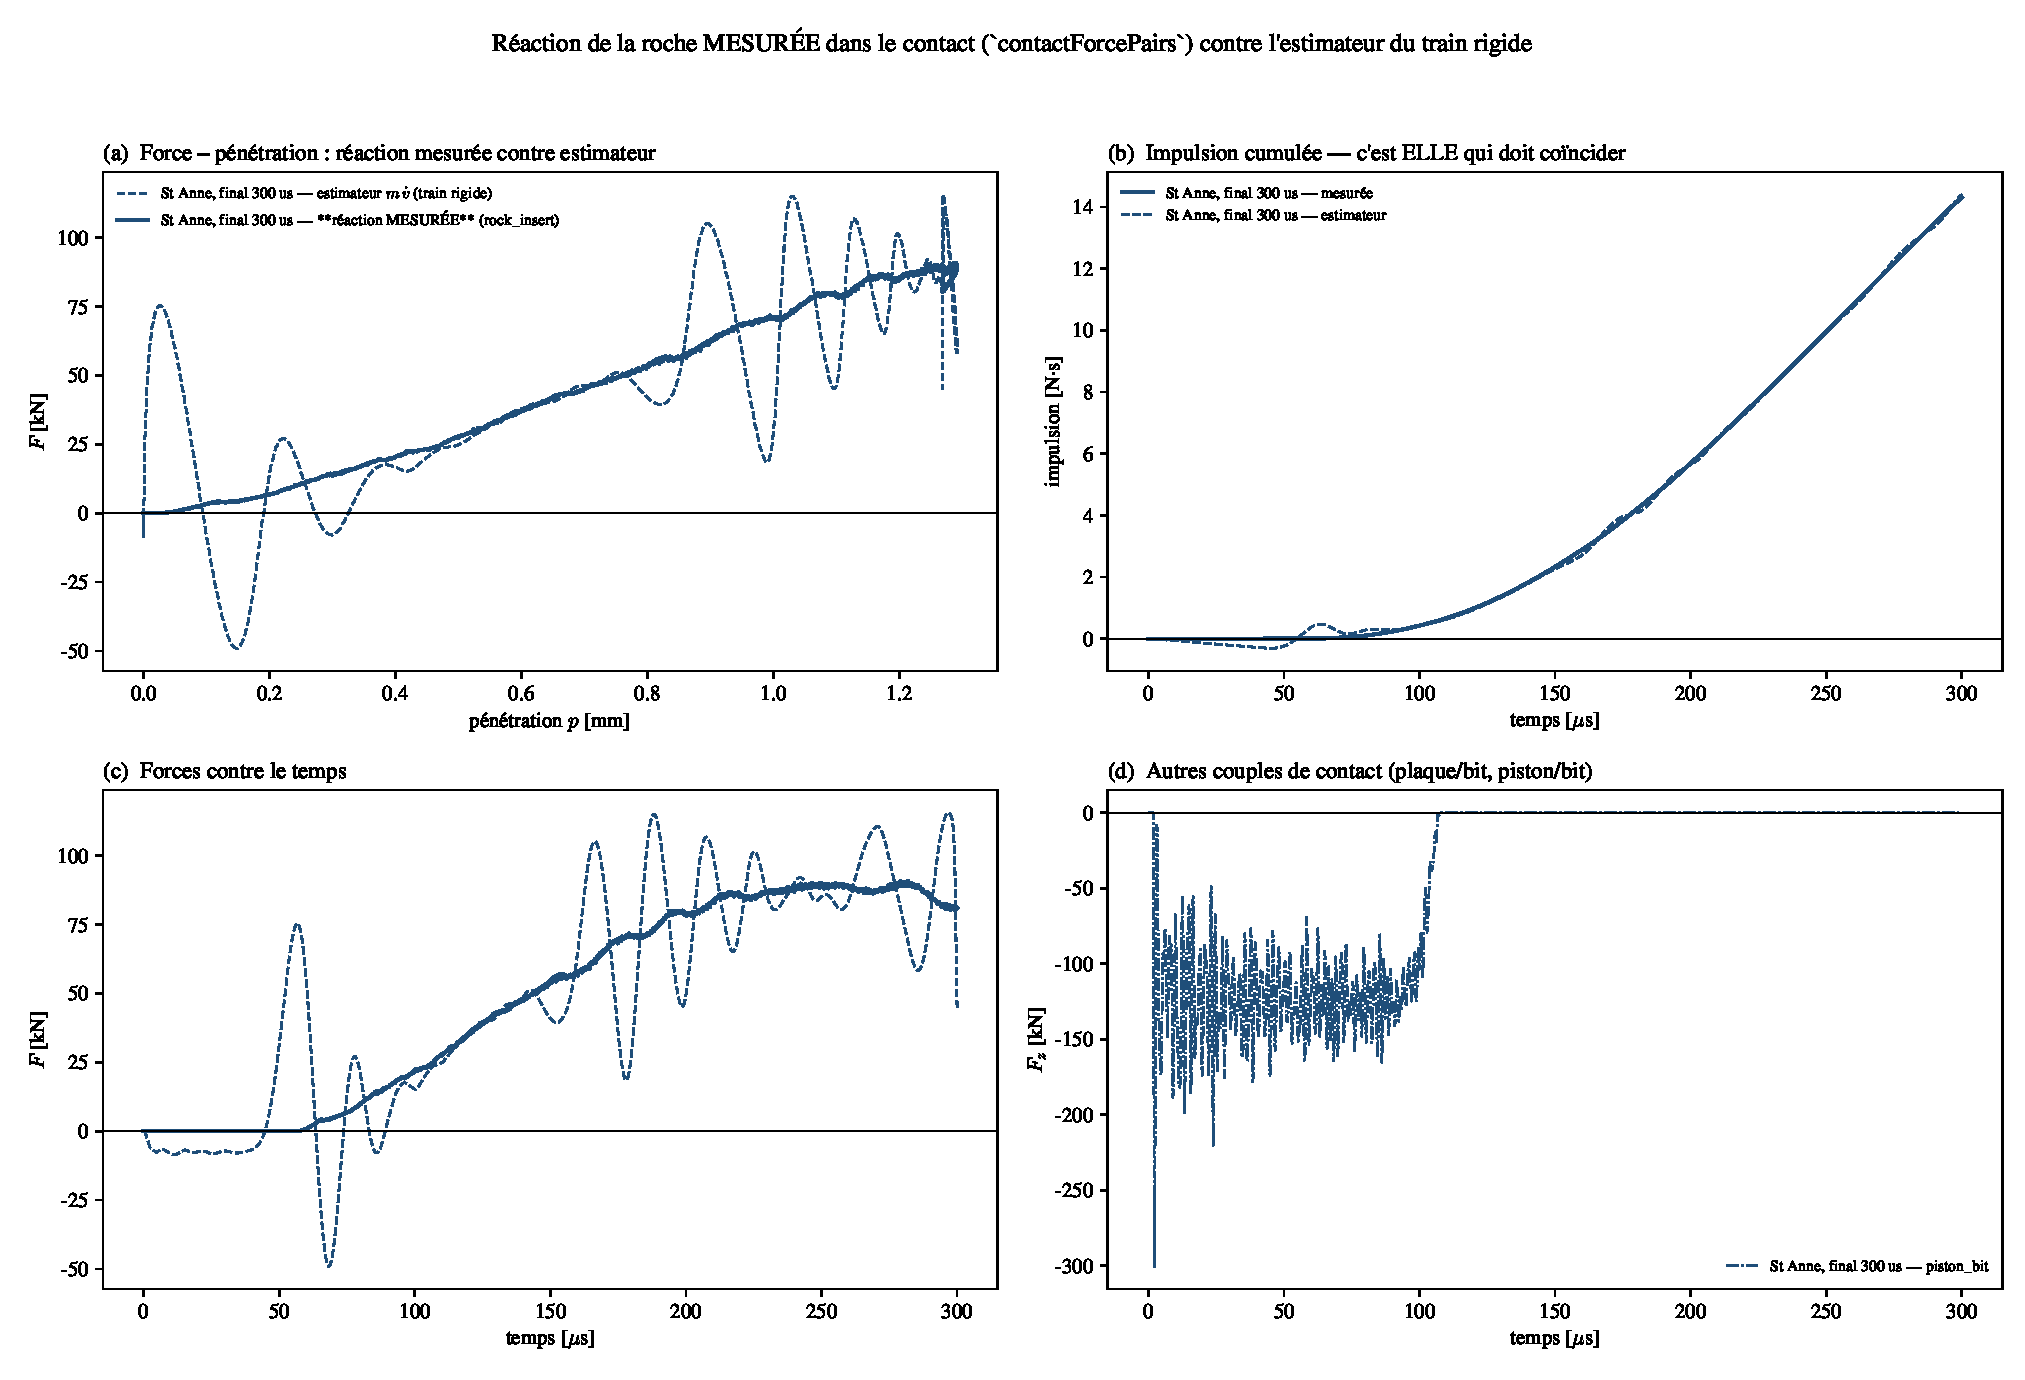
\includegraphics[width=\linewidth]{stanne_fp}
\caption{Réplique St Anne : force de contact insert-roche mesurée contre l'estimateur du train rigide, en fonction de la pénétration et du temps, impulsions cumulées et autres paires de contact.}
\label{fig-stanne-fp}
\end{figure}

Cette comparaison n'est pas indépendante du chemin de mise au point. La loi de joint et la pénalité ont été choisies pendant la même campagne, en regardant les critères de Yang et al. (\cle{vv/B_articles/README.md}, l.~256-260). Une seule résolution de maillage a tourné ; le maillage plus fin (251\,460 tétraèdres) reste à jouer. Les valeurs de référence elles-mêmes ne sont pas stables d'un document à l'autre : le bilan d'août citait une table de l'article avec une indentation de $9{,}40$ à $9{,}85$~m/s et un enfoncement de $1{,}53$~mm, que la comparaison de septembre, lue sur les figures 9 et 10, ne retrouve pas.

\subsection{Reproduction de Yang et al. 2026 : granite de Kuru}

L'impact sur le granite de Kuru à 9~m/s avec pulvérisation~\cite{yang2026pulverisation} était la cible initiale ; il a été délaissé au profit de St Anne parce que le modèle de pulvérisation n'est pas complètement publié. Il n'est pas reproduit (\cref{tab-kuru-ecarts}). La vitesse d'indentation est trop grande de $22~\%$, la pulvérisation quasi inactive (2 éléments contre environ 360), le freinage moyen trop faible, et le calcul s'arrête avant le retournement du bit.

\begin{table}[htbp]
\centering
\caption{Réplique Kuru, maillage $s = 1$ : grandeurs de rockim et de Yang et al. 2026.}
\label{tab-kuru-ecarts}
\begin{tabular}{@{}lrr@{}}
\toprule
grandeur & rockim & Yang et al. 2026 \\
\midrule
vitesse d'indentation, pente 10-$90~\%$ & $6{,}86$~m/s & $5{,}62$~m/s \\
compression maximale à la jauge & $175{,}95$~MPa & environ 160~MPa \\
éléments pulvérisés & 2 à $182{,}9~\mu$s & environ 360 \\
tétraèdres & 120\,185 & 230\,788 \\
masse du piston & $1{,}057$~kg & $1{,}173$~kg \\
freinage moyen & 20 à 25~kN (estimateur) & environ 57~kN (déduit) \\
\bottomrule
\end{tabular}
\end{table}

Les explications documentées sont partielles. La branche tangentielle de la loi de joint active n'était pas celle de Guo (pente $p_j$ au lieu de $2p_j$). La pulvérisation dépend d'une définition de la mesure de déformation que l'article ne donne pas. Les masses du train sont $10~\%$ plus faibles que chez Yang et al. Le freinage est comparé entre un maximum d'estimateur biaisé et une moyenne déduite. La chaîne causale qui irait d'un lit de débris trop lâche à une réaction faible, puis à l'absence de pulvérisation et de fissures radiales, est donnée par le document comme une hypothèse cohérente avec les données et non comme une causalité démontrée. Un diagnostic indépendant du 12 septembre conclut que les données ne démontrent pas une incapacité de la FDEM 3D à localiser la rupture, mais une reproduction encore non validée ; il a corrigé deux défauts de dépouillement (10~\% de faux positifs dans le décompte des joints rompus, rayon maximal pris pour une longueur de fissure).

La transcription mot à mot de la loi de joint de Solidity a établi que cette loi crée de l'énergie sur cycle fermé (\cref{sec-decharge}). Sur l'impact sans garde-fou, le travail cumulé des joints atteint 2\,745~J pour $31{,}5$~J apportés. Cela n'établit pas que la version interne du code de Yang et al. diverge de la même façon. Le code public de Solidity ne contient plus rien qui n'ait été transcrit : l'effet de vitesse interne, la pulvérisation, la configuration du granite et l'amortissement n'y figurent pas. Une demande de données aux auteurs est rédigée et n'a pas été envoyée.

\subsection{Autres comparaisons}

Sur la fracturation hydraulique en paroi de forage d'AbuAisha et al.~\cite{abuaisha2017hm}, calculée en 2D avec un couplage hydromécanique sans écoulement, la pression de rupture est trop forte de $+13{,}2~\%$ en isotrope et de $+24{,}9$ à $+25{,}0~\%$ en anisotrope ; l'ouverture d'une fissure mûre est à $-4~\%$ de Sneddon et le déplacement de paroi à $-2{,}0~\%$ de Lamé. Sur la compression simple 2D avec insertion adaptative de Yan et al.~\cite{yan2023adaptive}, la résistance de 51~MPa est retrouvée, ce qui reproduit leur simulation calée sans rien valider d'indépendant ; relancée avec le binaire courant, elle dérive de $+0{,}70~\%$ pour une tolérance de $0{,}29~\%$, avec $34~\%$ de joints rompus en plus, sans cause départagée entre l'évolution du code et le maillage de Voronoï. Sur le tunnel de Wang et al., le rayon de la zone endommagée vaut $17{,}19$~m contre 19~m. Ces comparaisons portent sur la simulation calée d'un autre code ou sur un critère analytique ; aucune n'est une validation au sens de la partie IV.

\subsection{Ce qui n'est pas validé}

Aucune comparaison n'a été faite à un essai qui n'a pas servi au calage, aucun essai dynamique de laboratoire (barres de Hopkinson, brésilien dynamique) n'a été confronté, et les données d'essai d'Aising et Gerbaud, base expérimentale des articles de Yang et al. et disponibles à Mines Paris-PSL, ne sont pas exploitées. Le modèle de pulvérisation n'est pas identifié. La loi \cle{plastic} n'est pas éprouvée hors des trajets testés. La convergence en maillage de la fissuration n'a qu'une résolution exploitable sur St Anne, et l'objectivité de la rupture vis-à-vis du maillage n'est pas quantifiée. Le relais du joint au contact n'est pas validé sur l'impact. L'énergie dissipée par la fissuration n'a jamais été comparée à $G_f$ multiplié par l'aire rompue.

\figaproduire{4.5cm}{écart relatif de chaque grandeur de comparaison (St Anne, Kuru, AbuAisha, Yan) à sa référence, avec le statut de la référence (simulation calée, essai, analytique) et la bande de dispersion expérimentale.}{aucun calcul nouveau ; agrégation des fichiers de résultats de \cle{vv/} et des tableaux de ce rapport, figure annoncée par \cle{vv/B_articles/README.md} mais absente.}

\section{Performances}
\label{sec-performances}

\subsection{Coût d'un calcul}

Le parallélisme est en mémoire partagée (OpenMP) : 21 régions parallèles dans le solveur FDEM 3D, 17 dans le solveur 2D, aucune dans les solveurs éléments finis 2D et éléments discrets. Les mesures de coût du dépôt sont prises sur des machines différentes, souvent partagées, et ne se comparent qu'en ordre de grandeur (\cref{tab-couts}). Le calcul St Anne de $300~\mu$s a demandé 29~h sur 14 fils. Le calcul Kuru le plus fin a demandé 15~h, quand Yang et al. annoncent 5~h pour un maillage deux fois plus fin, l'écart venant surtout du pas de temps ($1{,}0$ contre $2{,}5$~ns, \cref{sec-dt}).

\begin{table}[htbp]
\centering
\caption{Repères de coût relevés dans le dépôt.}
\label{tab-couts}
\begin{tabularx}{\linewidth}{@{}X r l@{}}
\toprule
cas & coût & statut \\
\midrule
FDEM 3D, 36\,000 tétraèdres et 70\,000 joints, 1 fil & 35~ms par pas & déclaré \\
FDEM 3D potentiel et adaptatif, 18 fils & $1{,}2~\mu$s par tétraèdre et par pas & mesuré \\
banc Kuru $s = 2{,}5$, 14 fils & $16{,}5$~ms par pas, dont $12{,}3$ de contact & mesuré \\
banc Kuru $s = 2{,}5$, $100~\mu$s, 4 fils & 398~s & mesuré \\
réplique Kuru $s = 1$, 120\,185 tétraèdres & 15~h & mesuré \\
réplique St Anne, 108\,667 tétraèdres, $300~\mu$s, 14 fils & 29~h~21 & mesuré \\
onde dans une barre, 20\,435 tétraèdres : éléments finis, FDEM adaptative, intrinsèque & 13, 539 et 1\,345~s & indicatif \\
\bottomrule
\end{tabularx}
\end{table}

\subsection{Gains mesurés}

L'activation adaptative du contact (13 août 2026) divise le temps d'une percussion 3D par $2{,}32$ avec des sorties identiques au bit, et celui d'une compression simple par $1{,}15$ (\cref{fig-gcact}). Le chantier de performance du contact par potentiel (14 août) l'a ramené de 682 à 448~s sur une percussion courte, toujours au bit près, mais il reste sept fois plus coûteux que la pénalité en régime de débris, au-delà de l'objectif de $1{,}3$ fixé. La parallélisation du potentiel (11 septembre) et la fusion parallèle des forces de joint (13 septembre), qui prenait $95~\%$ de son poste en série, ont rendu les calculs St Anne et Kuru abordables.

\begin{figure}[htbp]
\centering
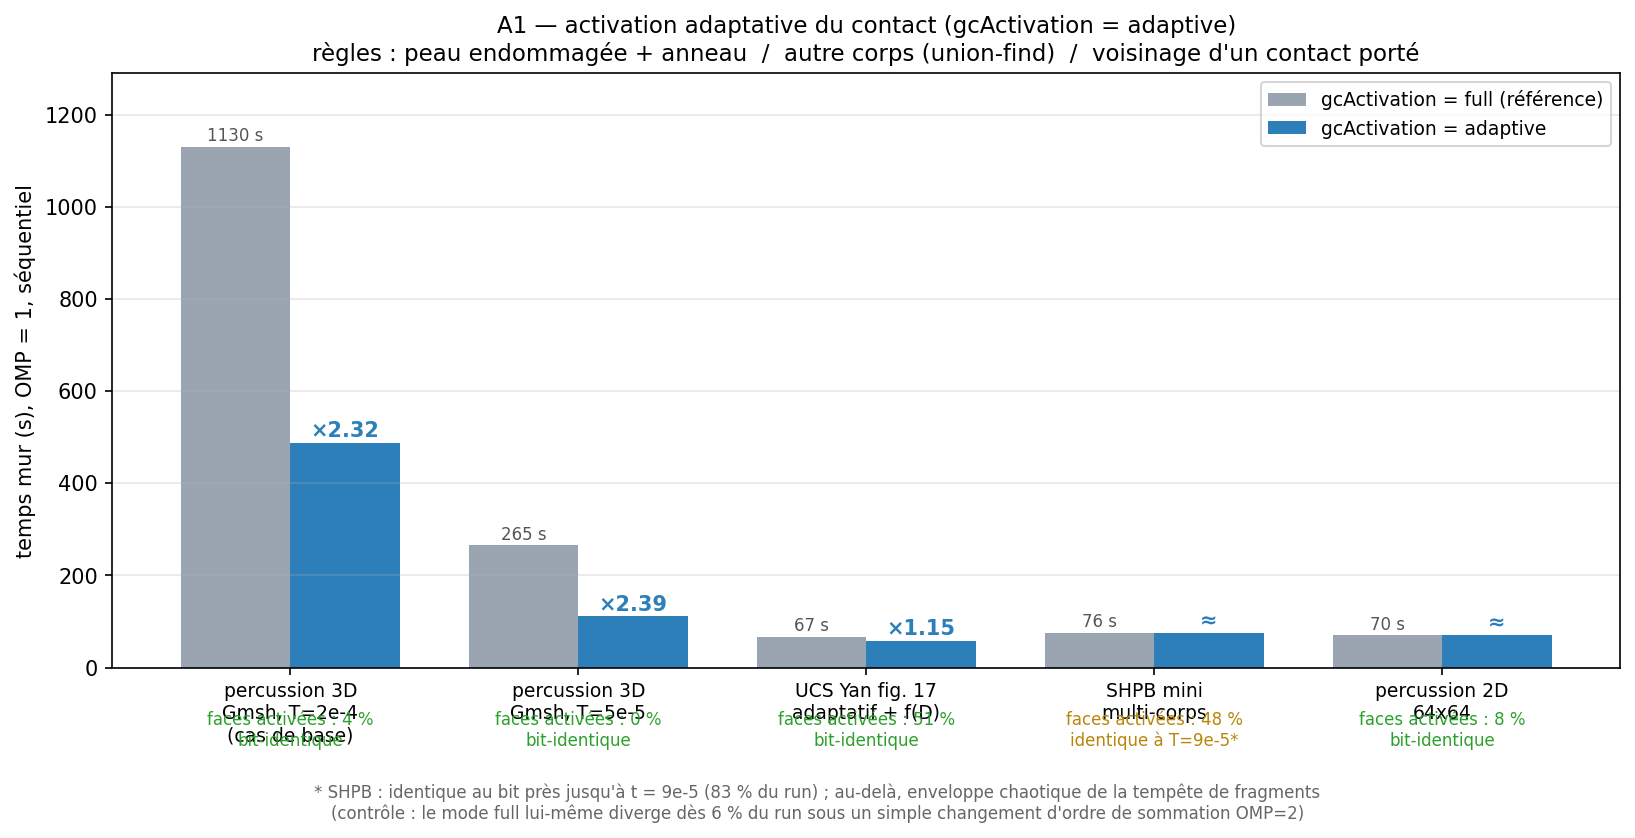
\includegraphics[width=0.8\linewidth]{gcactivation}
\caption{Temps de calcul avec et sans activation adaptative du contact sur cinq cas, à un fil, avec la part de faces activées.}
\label{fig-gcact}
\end{figure}

La campagne d'optimisation du 3 octobre 2026, à sorties identiques au bit, réduit le temps du banc Kuru court de $21~\%$ à un fil, $28~\%$ à 2 fils et $39~\%$ à 4 fils, et le poste du contact de $8{,}3$ à $2{,}7$~ms par pas ; les autres cas gagnent moins de $13~\%$. Deux options du même jour accélèrent au prix d'un changement de résultat : le pas variable réduit de $37~\%$ le temps d'une rupture adaptative et de $21~\%$ celui du banc Kuru, avec les mêmes joints rompus ; la force de contact par volume réduit de $36~\%$ le temps du banc Kuru, mais c'est une autre loi (\cref{tab-potvolume}).

Sur un Mac mini M4, le banc Kuru court passe de $49{,}8$ à $45{,}2$~s à un fil après optimisation, et de $24{,}6$ à $18{,}4$~s à 4 fils ; avec les deux options, $13{,}9$~s à 4 fils, soit un facteur $1{,}76$. Le passage de 4 à 10 fils ne rapporte que $14~\%$, à cause des six cœurs à basse consommation de cette machine et d'une répartition statique du travail. Ces chiffres sont écrits dans le journal des modifications ; le fichier de mesures que produit le script n'est pas versionné, et aucun profil par phase et par nombre de fils n'existe encore.

\subsection{Limites matérielles}

La spécification de performance (\cle{specs/001-pilier-performance-architecture/}) désigne le parallélisme CPU en mémoire partagée comme seule voie praticable sur le matériel disponible : la carte graphique du poste a une double précision bridée au 1/64, et le Mac a 16~Go de mémoire. Un cas de 842\,572 tétraèdres a été arrêté par la mémoire (7~Go, environ 700 octets d'état par élément). Aucune tâche de cette spécification n'est faite : il n'y a ni reprise sur point de sauvegarde, ni écriture VTU binaire.

\section{Limites connues et travaux en cours}
\label{sec-limites}

\subsection{Écarts non expliqués}

Sur St Anne, la masse de fragments est trop grande de $87~\%$ et l'enfoncement de $17~\%$, et le rebond n'est pas mesuré. Plus largement, aucun des 44 calculs d'impact archivés n'enregistre le retournement du bit de façon exploitable. Sur Kuru, la pulvérisation reste quasi inactive et le déficit de freinage n'est pas établi, faute d'une base de comparaison commune. Sur AbuAisha, la pression de rupture est trop forte de 13 à $25~\%$, avec des vitesses de particules 14 fois plus élevées que sur les figures de l'article. Sur Yan, la régression de la compression simple dérive sans cause attribuée.

\subsection{Options qui changent le résultat sans décision arrêtée}

Plusieurs options déplacent le résultat d'un impact et n'ont pas de valeur arrêtée par une étude ; un calcul de thèse doit fixer chacune et la citer (\cref{tab-options}).

\begin{table}[htbp]
\centering
\caption{Options qui changent le résultat d'un impact, effet mesuré et statut au 6 octobre 2026.}
\label{tab-options}
\begin{tabularx}{\linewidth}{@{}l X X@{}}
\toprule
option & effet mesuré & statut \\
\midrule
\cle{jointShearUnload} & \cle{solidity} crée de l'énergie ; \cle{origin} sans cliquet aussi & \cle{plastic} retenue le 14 septembre \\
\cle{jointPenaltyFactor} & onde ralentie de $(1 + 1{,}24/p_f)^{-1/2}$ & 20, puis 25, puis $26{,}3$ selon les comparaisons ; règle $p_f \geq 0{,}62/\varepsilon$ établie le 3 octobre \\
\cle{insertion} & cône broyé de 24~mm en intrinsèque, peau de 2~mm en adaptatif & sujet de thèse, non tranché \\
\cle{potForce} & pic $-7~\%$, impulsion $-16~\%$ en volume & une loi par étude \\
\cle{potStiffnessByPhase} & lit roche-roche dix fois plus souple avec \cle{min} & \cle{min} dans v3-P \\
raideur de contact de $E$ à $0{,}25\,E$ & force maximale $-5~\%$, ruptures $+13~\%$ & bancs seulement \\
\cle{meanTensionCapFactor} & plafond implicite à 3 fois $f_t$ & à poser à 0 dans les configurations de conformité \\
\cle{bulkModel} & non mesuré sur l'impact & co-rotationnel par défaut \\
\cle{dampingLocal} & tunnel 2D : $0{,}15$ à $0{,}7$ divise l'endommagement par 4 & ouvert \\
exposant de l'effet de vitesse & $1{,}516$ contre $1{,}847$ à 100~s$^{-1}$ & $0{,}17$ retenu \\
\bottomrule
\end{tabularx}
\end{table}

\subsection{Chantiers ouverts}

La campagne de vérification et validation doit jouer les sept bancs préparés, environ 7~h à 2 fils pour les cas par défaut, et ouvrir les parties III et IV. La réplique St Anne doit être prolongée à $500~\mu$s pour mesurer le rebond et rejouée sur le maillage fin pour sa convergence. Le programme d'accélération a ses étapes suivantes écrites : profil par phase, combinaisons d'options, stabilité de la pénalité de contact des joints selon Ghesquière-Diérickx et al.~\cite{ghesquiere2025}, dont le défaut serait instable d'après cet article sans que le micro-banc de rockim ne le montre. La branche de développement n'est pas fusionnée, n'a pas de demande de fusion et n'a pas été compilée sous Windows.

\subsection{Ce qui manque pour la thèse}

La thèse a besoin d'une comparaison complète à au moins un article, rebond compris, avec une étude de convergence en maillage. Elle a besoin de données d'essai indépendantes du calage ; les essais d'Aising et Gerbaud, internes à Mines Paris-PSL, sont la candidate naturelle, et la feuille de route les classait comme bloquants pour toute validation. Elle a besoin de relier les deux chemins de calage, le triaxial du Red Bohus et l'impact du Kuru, qui aujourd'hui ne se croisent pas. Elle a besoin que la campagne de vérification et validation soit jouée jusqu'à ses verdicts.

Deux questions de pérennité restent ouvertes. Le dépôt public n'a pas de licence alors qu'il contient des parties transcrites d'un code sous LGPL. Une seule personne connaît le code, et sa documentation de référence, longue de 3\,200 lignes, contient des passages périmés relevés dans ce rapport : nombre de tests, comportement des clés inconnues, valeur par défaut du plafond de traction, chiffres de création d'énergie de la loi de Solidity, statut de la spécification de l'impact.


\appendix
\section{Équations principales}
\label{sec-annexe-equations}

\subsection{Volume}

Élasticité co-rotationnelle, avec $\mathbf R$ la rotation extraite de $\mathbf F$ :
\[
\boldsymbol\varepsilon = \operatorname{sym}(\mathbf R^{\mathsf T}\mathbf F) - \mathbf I, \qquad
\boldsymbol\sigma = \lambda \operatorname{tr}\boldsymbol\varepsilon\, \mathbf I + 2\mu\boldsymbol\varepsilon .
\]
Loi néo-hookéenne de Guo, avec $J = \det\mathbf F$ et $\mathbf B = \mathbf F\mathbf F^{\mathsf T}$ :
\[
\mathbf T = \frac{\mu}{J}(\mathbf B - \mathbf I) + \frac{\lambda}{J}\ln J\, \mathbf I .
\]
Pulvérisation de Yang et al. 2026, avec $\delta_m = h\,\varepsilon_{vm}$ :
\[
\boldsymbol\sigma = C_d (1 - D)\bar{\boldsymbol\sigma}, \qquad
D = D_\text{max}\, \frac{\delta_m - \delta_0}{\delta_F - \delta_0} \in [0, D_\text{max}] .
\]

\subsection{Joints cohésifs}

Pénalité et souplesse nominale :
\[
p_j = \frac{p_f E}{h}, \qquad E_\text{eff} = \frac{E}{1 + 1/p_f}, \qquad
\frac{c_\text{eff}}{c} = \Big(1 + \frac{\alpha}{p_f}\Big)^{-1/2},\ \alpha = 1{,}239 \text{ (mesuré)} .
\]
Branche élastique parabolique de Guo, avec $r = \delta_n/\delta_{nE}$ et $\delta_{nE} = f_t/p_j$ :
\[
\sigma = f_t (2r - r^2) \ \ (\delta_n \geq 0), \qquad \sigma = 2 p_j \delta_n \ \ (\delta_n < 0) .
\]
Enveloppe de cisaillement de Yang et al. :
\[
f_s = c - \tan\varphi\, \min(\sigma_n, f_t) .
\]
Courbe d'adoucissement en z de Munjiza, avec $a = 0{,}63$, $b = 1{,}8$, $c = 6$ et $\int_0^1 f = 0{,}386$ :
\[
f(D) = \Big[1 - \frac{a+b-1}{a+b} \exp\Big(\frac{D(a+cb)}{(a+b)(1-a-b)}\Big)\Big]\big[a(1-D) + b(1-D)^c\big] .
\]
Mode mixte et énergies :
\[
D = \sqrt{r_n^2 + r_s^2}, \qquad G_I = f_t\, \delta_t \int_0^1 f, \qquad G_{II} = c\, \delta_s \int_0^1 f .
\]
Frottement résiduel du joint :
\[
\mu_\text{eff} = \mu_\text{res} + (\tan\varphi - \mu_\text{res})\, f(D) .
\]
Décharge \cle{plastic}, retour radial :
\[
\tau_\text{essai} = p_j(\delta_s - s_p), \qquad |\tau_\text{essai}| > \tau_\text{lim} \Rightarrow \tau = \tau_\text{lim}\, \frac{\tau_\text{essai}}{|\tau_\text{essai}|} .
\]
Décharge \cle{origin}, sécante à l'origine, et énergie créée par cycle à glissement fixé entre deux raideurs sécantes :
\[
\tau = \min\big(p_j s_\text{max}, \tau_\text{lim}(\sigma_n)\big)\, \frac{s}{s_\text{max}}, \qquad \Delta W = \tfrac12 (k_2 - k_1) s^2 .
\]
Effet de la vitesse de déformation :
\[
DIF_t = \min\big(1{,}85;\ 0{,}95 + 0{,}41\,\dot\varepsilon^{a_t}\big), \qquad
DIF_c = \min\big(1{,}84;\ 0{,}77 + 0{,}56\,\dot\varepsilon^{0{,}07}\big) .
\]
Effet d'échelle :
\[
f_t \leftarrow f_t\, (Z_\text{eff}/V_J)^{1/m} .
\]

\subsection{Contact}

Potentiel de Munjiza, avec $\lambda_k$ les coordonnées barycentriques :
\[
\varphi = 4 \min_k \lambda_k, \qquad
\mathbf F_A = p \int_{A\cap B} (\nabla\varphi_A - \nabla\varphi_B)\, dV = p \oint_{\partial(A\cap B)} (\varphi_A - \varphi_B)\, \mathbf n\, d\Gamma, \qquad \mathbf F_B = -\mathbf F_A .
\]
Force par volume de recouvrement de Liu et al. :
\[
\Phi = \tfrac12 k_n \frac{V^2}{V'}, \qquad V' = \frac{2 V_A V_B}{V_A + V_B}, \qquad
\mathbf F_A = -\frac{k_n V}{V'} \sum_{i} a_i \mathbf n_i .
\]
Frottement incrémental :
\[
\mathbf F_t^{n+1} = \Pi_\perp \mathbf F_t^{n} - k_t \Delta t\, \mathbf v_t, \qquad \|\mathbf F_t^{n+1}\| \leq \mu_{AB} F_n, \qquad \mu_{AB} = \min(\mu_A, \mu_B) .
\]
Naissance en rampe et naissance calée sur la force du joint mort :
\[
s = \max\Big(0, 1 - \frac{V_\text{ref}}{V}\Big),\ V_\text{ref} \leftarrow V_\text{ref}\, e^{-\Delta t/\tau} ; \qquad
s = \operatorname{clamp}\Big(\frac{|f_\text{mort}|}{\|\mathbf F\|};\ 0{,}01;\ 3\Big) .
\]
Couplage endommagement-contact :
\[
d = \min(1 - D_i, 1 - D_j), \quad d \leftarrow 10^{-3} d \text{ si } d < 0{,}041, \qquad F_n \leftarrow d\, F_n, \ \mu \leftarrow d\, \mu .
\]
Contact d'outil en vitesse au nœud $i$ :
\[
v_n = \Big(\mathbf v_i + \frac{\Delta t}{m_i}\mathbf f_i - \mathbf v_\text{outil}\Big)\cdot\mathbf n, \qquad
r_n = m_i\Big(\rho \frac{g}{\Delta t} - v_n\Big) \text{ si contact}, \qquad \|\mathbf r_t\| \leq \mu r_n .
\]

\subsection{Pas de temps et mise en données}

\[
\Delta t = f_{\Delta t} \min\Big( \min_i 2\sqrt{\frac{m_i}{K_i + n_\text{extra} k_p}},\ \frac{h_\text{insc,min}}{c_{p,\text{max}}},\ \frac{\rho h^2}{4\mu} \Big),
\]
\[
t_0 = \frac{\text{jeu}}{v}, \qquad t_c \approx 2{,}87 \Big(\frac{m^2}{R E^{*2} v}\Big)^{1/5}, \qquad
2\,\Delta x < \ell_{cz} = \frac{E G_f}{f_t^2} < a = \sqrt{R\delta} .
\]

\subsection{Bilan d'énergie}

\begin{multline*}
E_c(t) - E_c(0) = W_\text{él} + W_\text{joints} + W_\text{amort} + W_\text{contact} + W_\text{Cundall} \\
+ W_\text{front} + W_\text{outil} + W_\text{vol} + W_\text{intégr} + r,
\qquad W_\text{intégr} = \sum_{\text{pas}} \sum_i \frac{f_i^2 \Delta t^2}{2 m_i} .
\end{multline*}

\section{Clés de configuration utilisées dans la thèse}
\label{sec-annexe-cles}

Le tableau rassemble les clés qui fixent la physique d'un impact FDEM 3D, avec leur défaut et leur réglage dans la configuration v3-P du banc Kuru. La référence complète des clés est \cle{DOCUMENTATION_rockim.md} ; chaque calcul écrit dans \cle{config_effective.cfg} toutes les valeurs qu'il a utilisées.

\begin{longtable}{@{}p{0.34\linewidth} p{0.22\linewidth} p{0.36\linewidth}@{}}
\caption{Clés de l'impact FDEM 3D, défaut et réglage v3-P.}\label{tab-cles}\\
\toprule
clé & défaut & v3-P \\
\midrule
\endfirsthead
\toprule
clé & défaut & v3-P \\
\midrule
\endhead
\bottomrule
\endfoot
\cle{mode} & sans objet & \cle{fdem3d} \\
\cle{mesh} & grille & \cle{file}, six corps nommés \\
\cle{toolShape} & sphère & \cle{none} \\
\cle{groupBond.bit.insert} & aucun & \cle{joints} \\
\cle{groupContinuum.<corps>} & aucun & métaux \\
\cle{insertion} & \cle{intrinsic} & \cle{intrinsic} \\
\cle{jointPenaltyFactor} & 20 & 20 \\
\cle{jointPenaltyLength} & \cle{min} & \cle{min} \\
\cle{jointElastic} & linéaire & \cle{parabolic} \\
\cle{jointNormalProxy} & historique & \cle{law} \\
\cle{jointSoftening} & \cle{linear} & \cle{munjiza} \\
\cle{jointShearEnvelope} & \cle{yan} & \cle{yang} \\
\cle{jointShearRange} & \cle{cohesion} & \cle{coulomb} \\
\cle{jointShearUnload} & \cle{plastic} & \cle{plastic} \\
\cle{jointSecantRatchet} & désactivé & \cle{on} \\
\cle{jointResidualMu} & non posée & 0 \\
\cle{jointDeath} & \cle{separation} & \cle{damage} \\
\cle{jointFailRule} & \cle{any} & \cle{majority} \\
\cle{jointQuadrature} & \cle{vertex} & \cle{midedge} \\
\cle{jointDeltaC} & \cle{exact} & \cle{solidity} \\
\cle{jointXi} & $0{,}05$ & 0 \\
\cle{bulkModel} & co-rotationnel & co-rotationnel \\
\cle{bulkDamage} & désactivé & \cle{yang} \\
\cle{bulkDamagePhase} & toutes & \cle{rock} \\
\cle{meanTensionCapFactor} & 3 & non posée, donc 3 \\
\cle{strainRateDIF} & désactivé & \cle{yang}, exposant $0{,}17$ en traction \\
\cle{strainRateDIFArm} & selon l'insertion & \cle{continuous} \\
\cle{strainRateFilter} & passe-bas & \cle{none} \\
\cle{contact} & \cle{penalty} & \cle{potential} \\
\cle{potForce} & \cle{munjiza} & \cle{munjiza} \\
\cle{potStiffnessByPhase} & \cle{max} & \cle{min} \\
\cle{potTangentFactor} & 1 & $1{,}4286$ \\
\cle{gcActivation} & \cle{full} & \cle{adaptive} \\
\cle{gcBirth} & \cle{ramp} & \cle{ramp} \\
\cle{contactMu.rock} & $0{,}5$ & $0{,}18$ \\
\cle{contactDamageCoupling} & \cle{off} & \cle{solidity} \\
\cle{dampingLocal} & $0{,}05$ & 0 \\
\cle{dtFactor} & $0{,}15$ & $0{,}15$ \\
\cle{energyBodyForces} & désactivé & \cle{on} \\
\cle{budgetAbortPct} & désactivé & 2 \\
\cle{groupVel.piston} & aucune & 9~m/s vers le bas \\
\end{longtable}

\section{Reproduire les résultats de ce rapport}
\label{sec-annexe-reproduire}

\subsection{Compiler et lancer}

rockim se compile avec CMake sous Linux, macOS ou Windows ; Eigen est téléchargé s'il n'est pas installé et OpenMP est détecté s'il existe (\cle{GUIDE_rockim.md}, §2). Un calcul se lance par \cle{rockim <configuration> <dossier de sortie>}, le nombre de fils se fixant par la variable \cle{OMP_NUM_THREADS}. Un seul fil donne des sorties identiques au bit au calcul série. La variable \cle{ROCKIM_PROF=1} imprime le coût de chaque phase du pas.

\subsection{Vérification}

La suite se lance depuis la racine du dépôt par \cle{python tools/verify_suite.py --tier fast}, ou \cle{full} et \cle{all} pour les niveaux supérieurs, à un fil par défaut. Les auto-tests se lancent par \cle{rockim selftest-<nom>}. L'identité au bit se contrôle par \cle{python tools/bitid.py}, à 4 fils.

\subsection{Bancs de validation}

Chaque banc de \cle{vv/} se lance par \cle{python vv/<banc>/<script>.py all}, qui prépare les maillages et les configurations, lance les calculs et écrit \cle{resultats.json} et les figures \cle{fig_*.pdf}. Les actions \cle{prepare}, \cle{run} et \cle{analyse} se lancent aussi séparément. Le lanceur \cle{vv/run_daemon.py} prend en charge les bancs marqués prêts et respecte un plafond global de processus.

\subsection{Provenance des figures}

\begin{longtable}{@{}p{0.3\linewidth} p{0.64\linewidth}@{}}
\toprule
figure & source \\
\midrule
\endhead
\cref{fig-montage} & \cle{results/fig/config_stanne/montage.png} \\
\cref{fig-hertz} & \cle{figures_impact/hertz_compare.png}, script \cle{plot_hertz.py} \\
\cref{fig-V1conv,fig-V1pen} & \cle{vv/V1_onde/}, script \cle{viz_v1.py} \\
\cref{fig-P21} & \cle{vv/P2_bloc/p2_bloc.py} \\
\cref{fig-stanne-joints,fig-stanne-fp} & \cle{results/fig/stanne300/}, scripts \cle{tools/fig_joints_only.py} et \cle{tools/fig_fp.py} \\
\cref{fig-gcact} & \cle{A1_gcactivation.png} à la racine du dépôt \\
\bottomrule
\end{longtable}

Les figures géométriques du calcul St Anne demandent les trames VTU, environ 2~Go, qui ne sont pas dans le dépôt. Les fichiers \cle{.odb} et les grands résultats bruts vivent sur le poste du doctorant.

\subsection{Les documents de référence}

Pour approfondir un point, l'ordre de lecture recommandé est le suivant : \cle{GUIDE_rockim.md} pour l'usage, \cle{DOCUMENTATION_rockim.md} pour la référence des clés et des lois, \cle{docs/VV_campagne.md} pour la campagne de vérification et validation, \cle{docs/COMPARAISON_yang2025_stanne_2026-09-14.md} pour la réplique St Anne, \cle{docs/ECARTS_guo2014_rockim_2026-09-13.md} pour la transcription de Solidity, \cle{HANDOFF_2026-10-03.md} pour l'état le plus récent.


\printbibliography[heading=bibintoc,title={Références}]

\end{document}
